\documentclass[11pt]{article}
\usepackage{amsmath, amssymb, amscd, amsthm, amsfonts}
\usepackage{graphicx}
\usepackage{hyperref}

\usepackage{subcaption}

\oddsidemargin 0pt
\evensidemargin 0pt
\marginparwidth 40pt
\marginparsep 10pt
\topmargin -20pt
\headsep 10pt
\textheight 8.7in
\textwidth 6.65in
\linespread{1.2}

\title{Design and Implementation of Quantum Repeaters: Insights on Quantum Entanglement Purification}
\author{Karoki A. Mugambi and Geoffrey O. Okeng'o}
\date{%
    The Astrophysics and Space Science Research Group, Department of Physics, Faculty of Science and Technology, University of Nairobi, Kenya.\\[2ex]%
    % \today
}

\newtheorem{theorem}{Theorem}
\newtheorem{lemma}[theorem]{Lemma}
\newtheorem{conjecture}[theorem]{Conjecture}

\newcommand{\rr}{\mathbb{R}}

\newcommand{\al}{\alpha}
\DeclareMathOperator{\conv}{conv}
\DeclareMathOperator{\aff}{aff}

\begin{document}

\maketitle

\begin{abstract}
Quantum communication is an upcoming new technology that is driving the future of information transmission and communication technologies to a new paradigm. It relies on quantum entanglement to facilitate transmission of quantum states between parties. Quantum repeaters are employed to facilitate long-distance transmission. They extend the transmission range by fragmenting the channel into multiple small segments where they perform entanglement swapping between each segment endpoints until the sender and receiver become entangled, forming a complete quantum link for communication. This research focuses on quantum entanglement purification, the protocol that ensures entangled states maintain a high fidelity above the communication channel operational threshold. Our study gives insight into the optimum purification strategy by determining at what stage the purification protocol should be executed. Moreover, optimization schemes were applied to evaluate the effects of various purification protocols. IBM Qiskit was used for the circuit implementation and simulation. The results provide a guide into future approaches to implementing practical quantum repeaters and the challenges existing and those bound to arise.
\end{abstract}


\section{Introduction}
Quantum communication leverages the principles of quantum mechanics to transmit quantum information between remote locations. The quantum information is encoded in a qubit - the basic unit of quantum information.

At the core of quantum communication is the principle of quantum entanglement, which gives rise to the phenomena of quantum teleportation as a new paradigm protocol for communication \cite{Bennett_1993}.

Currently, active experimental works in quantum communication channels are carried out either in optical fibres or free space, both of which are affected by noise during transmission. The photon intensity is attenuated exponentially with transmission distance \cite{Ruihong_2019}. This limits long-distance communication channels. Quantum repeaters were introduced to overcome this long-distance limitation \cite{Briegel_1998}.

Quantum repeaters are devices that extend the range of quantum channels. They do so by fragmenting communication channels into small segments composed of nodes or relay stations, each with a quantum repeater that teleports entangled states between adjacent nodes. We note that the terms nodes, relay stations and stations are here used interchangeably and imply the same thing unless otherwise stated. The length of the segments is chosen such that it is less than the attenuation length of the channel \cite{Das_2021}. Entanglement is established between adjacent nodes using quantum entanglement switching protocol, eventually forming a large-scale quantum link from the sender to the receiver station \cite{Gisin_2007, Ruihong_2019}.

The main components of a quantum repeater include; quantum entanglement switching for swapping entangled states between adjacent nodes, quantum memory for storing quantum states for efficient on demand retrieval and quantum entanglement purification for enhancing the fidelity of the entangled states. These components have a few limitations arising from imperfections in the source of entangled particles, the quantum operations involved and the interconnecting communication channels \cite{Herbst_2015}.

Despite these limitations, quantum repeaters have been successfully demonstrated in experiments, such as Herbst et al., who managed to use a quantum repeater to teleport an entangled state, a photon, between the Canary islands of La Palma to Tenerife, a distance of about 143 km \cite{Herbst_2015}. The entanglement swapping experiment used two polarization-entangled photon pairs generated in two identical spontaneous parametric down-conversion (SPDC) sources using a non-linear crystal, $\beta$-barium borate (BBO) \cite{Herbst_2015}.

% Each station has a quantum memory to store the entangled state before being used in the entanglement switching protocol.
Quantum entanglement purification protocol is a key component in quantum repeaters, necessary in first generation or near-term quantum repeaters \cite{Muralidharan2016}. It is essential in ensuring entangled states maintain high fidelity throughout the transmission \cite{Bennett_1996}, thereby compensating for loss of fidelity due to noise or imperfections in the communication channel.

The two purification protocols employed in this research are: Bennett's protocol \cite{Bennett_1996} and Deutsch's protocol \cite{Deutsch_1996}.

Performance aspects considered for the purification protocols are; fidelity of the purified Bell pair, success probability and circuit length \cite{Krastanov2019optimized}. All protocols work towards obtaining shorter circuits, achieving higher success rates and better final fidelities \cite{Krastanov2019optimized}.

Quantum repeaters are necessary for future quantum communication technologies such as quantum internet \cite{Gisin_2007, Briegel_1998}. They will extend the range of transmission links to inter-continental global scale, powering the future of a global quantum network.

However, implementing them in the real world is a huge technological challenge. There is a lot of ongoing research into the individual components and full-scale architecture of a quantum repeater.

This research paper presents the full-scale architecture of a quantum repeater designed and implemented using quantum circuits executed on a quantum computer. We used the said quantum repeater implementation to study quantum entanglement purification.
%%%%%%%%%%%%%%%%%%%%%%%%%%%%%%%%%%%%%%%%%%%%%%%%%%%%
%%%%%%%%%%%%%%%%%%%%%%%%%%%%%%%%%%%%%%%%%%%%%%%%%%%%
\section{Experimental Setup}

\subsection{Research Approach}
This research paper presents a theoretical and computational approach. The architectural design of the quantum repeater is modelled based on the use of quantum optics as opposed to earth to satellite links. The conceptual implementation is however, the same.

This study uses IBM quantum computers and IBM Qiskit library. The environment exposed to superconducting qubits in the IBM quantum computers can ideally emulate the same environment quantum repeaters will be exposed to when in real-world operation \cite{Das_2021}.

% \subsection{Design and Implementation Approach}
Each execution stage and protocol of the quantum repeater was translated into a modular quantum circuit that was independently executed on IBM Qiskit. The modularity of the code helped test out different purification strategies, protocols and components of the quantum repeater for better analysis. The quantum circuits were first executed on the native simulation - IBM Qiskit's QASM simulator - before being finally executed on actual IBM quantum computers.

Performance analysis was done based on the fidelity of the purified Bell pair. Optimisation schemes were applied to the entanglement purification circuits to analyse their performance.

\subsection{Entanglement Generation}
The circuit implementation that prepares and generates an entangled pair takes as input two qubits and performs Hadamard and Controlled-NOT unitary gate operations on them. Each EPR pair gets distributed to adjacent nodes. For instance, one pair, $|\Phi^{+}\rangle_{AB}$ gets to entangles A and B while the other pair, $|\Phi^{+}\rangle_{CD}$ gets to entangles C and D.

\subsection{Quantum Entanglement Distribution}
The first distribution is that of the EPR pairs $|\Phi^{+}\rangle_{AB}$ and $|\Phi^{+}\rangle_{CD}$ to their respective nodes, each node taking one of the qubits from a pair. The distribution stage that involves the quantum repeater requires the distribution of entanglement along the transmission line from sender to receiver. This entanglement distribution relies on quantum memories, entanglement purification protocols and entanglement swapping protocols to distribute entanglement between nodes from the start of the communication link to the end.

\subsection{Quantum Memory}
The entangled state $|\Phi^{+}\rangle_{AB}$ is momentarily stored in a quantum memory and only retrieved when it is needed to perform entanglement distribution between nodes B and C to get the entangled state $|\Phi^{+}\rangle_{BC}$.

\subsection{Quantum Entanglement Purification}
We constrained this research to the two common purification protocols: Bennett's protocol \cite{Bennett_1996} and Deutsch's protocol \cite{Deutsch_1996}. Each protocol has its own complexity of implementation. They also provide varying fidelity levels and produce varying degrees of overhead during circuit operation.

Successful purification using these protocol gives measurement results as $|00\rangle$ or $|11\rangle$. Any other measurement result, either $|01\rangle$ or $|10\rangle$, indicates a failed purification operation, upon which the purification protocol needs a fresh restart.

Figure \ref{fig:purification_bennett} and Figure \ref{fig:purification_deutsch} show the implementation of the two purification protocols.
\begin{figure}[ht]
  \centering
  \begin{subfigure}[b]{0.62\textwidth}
    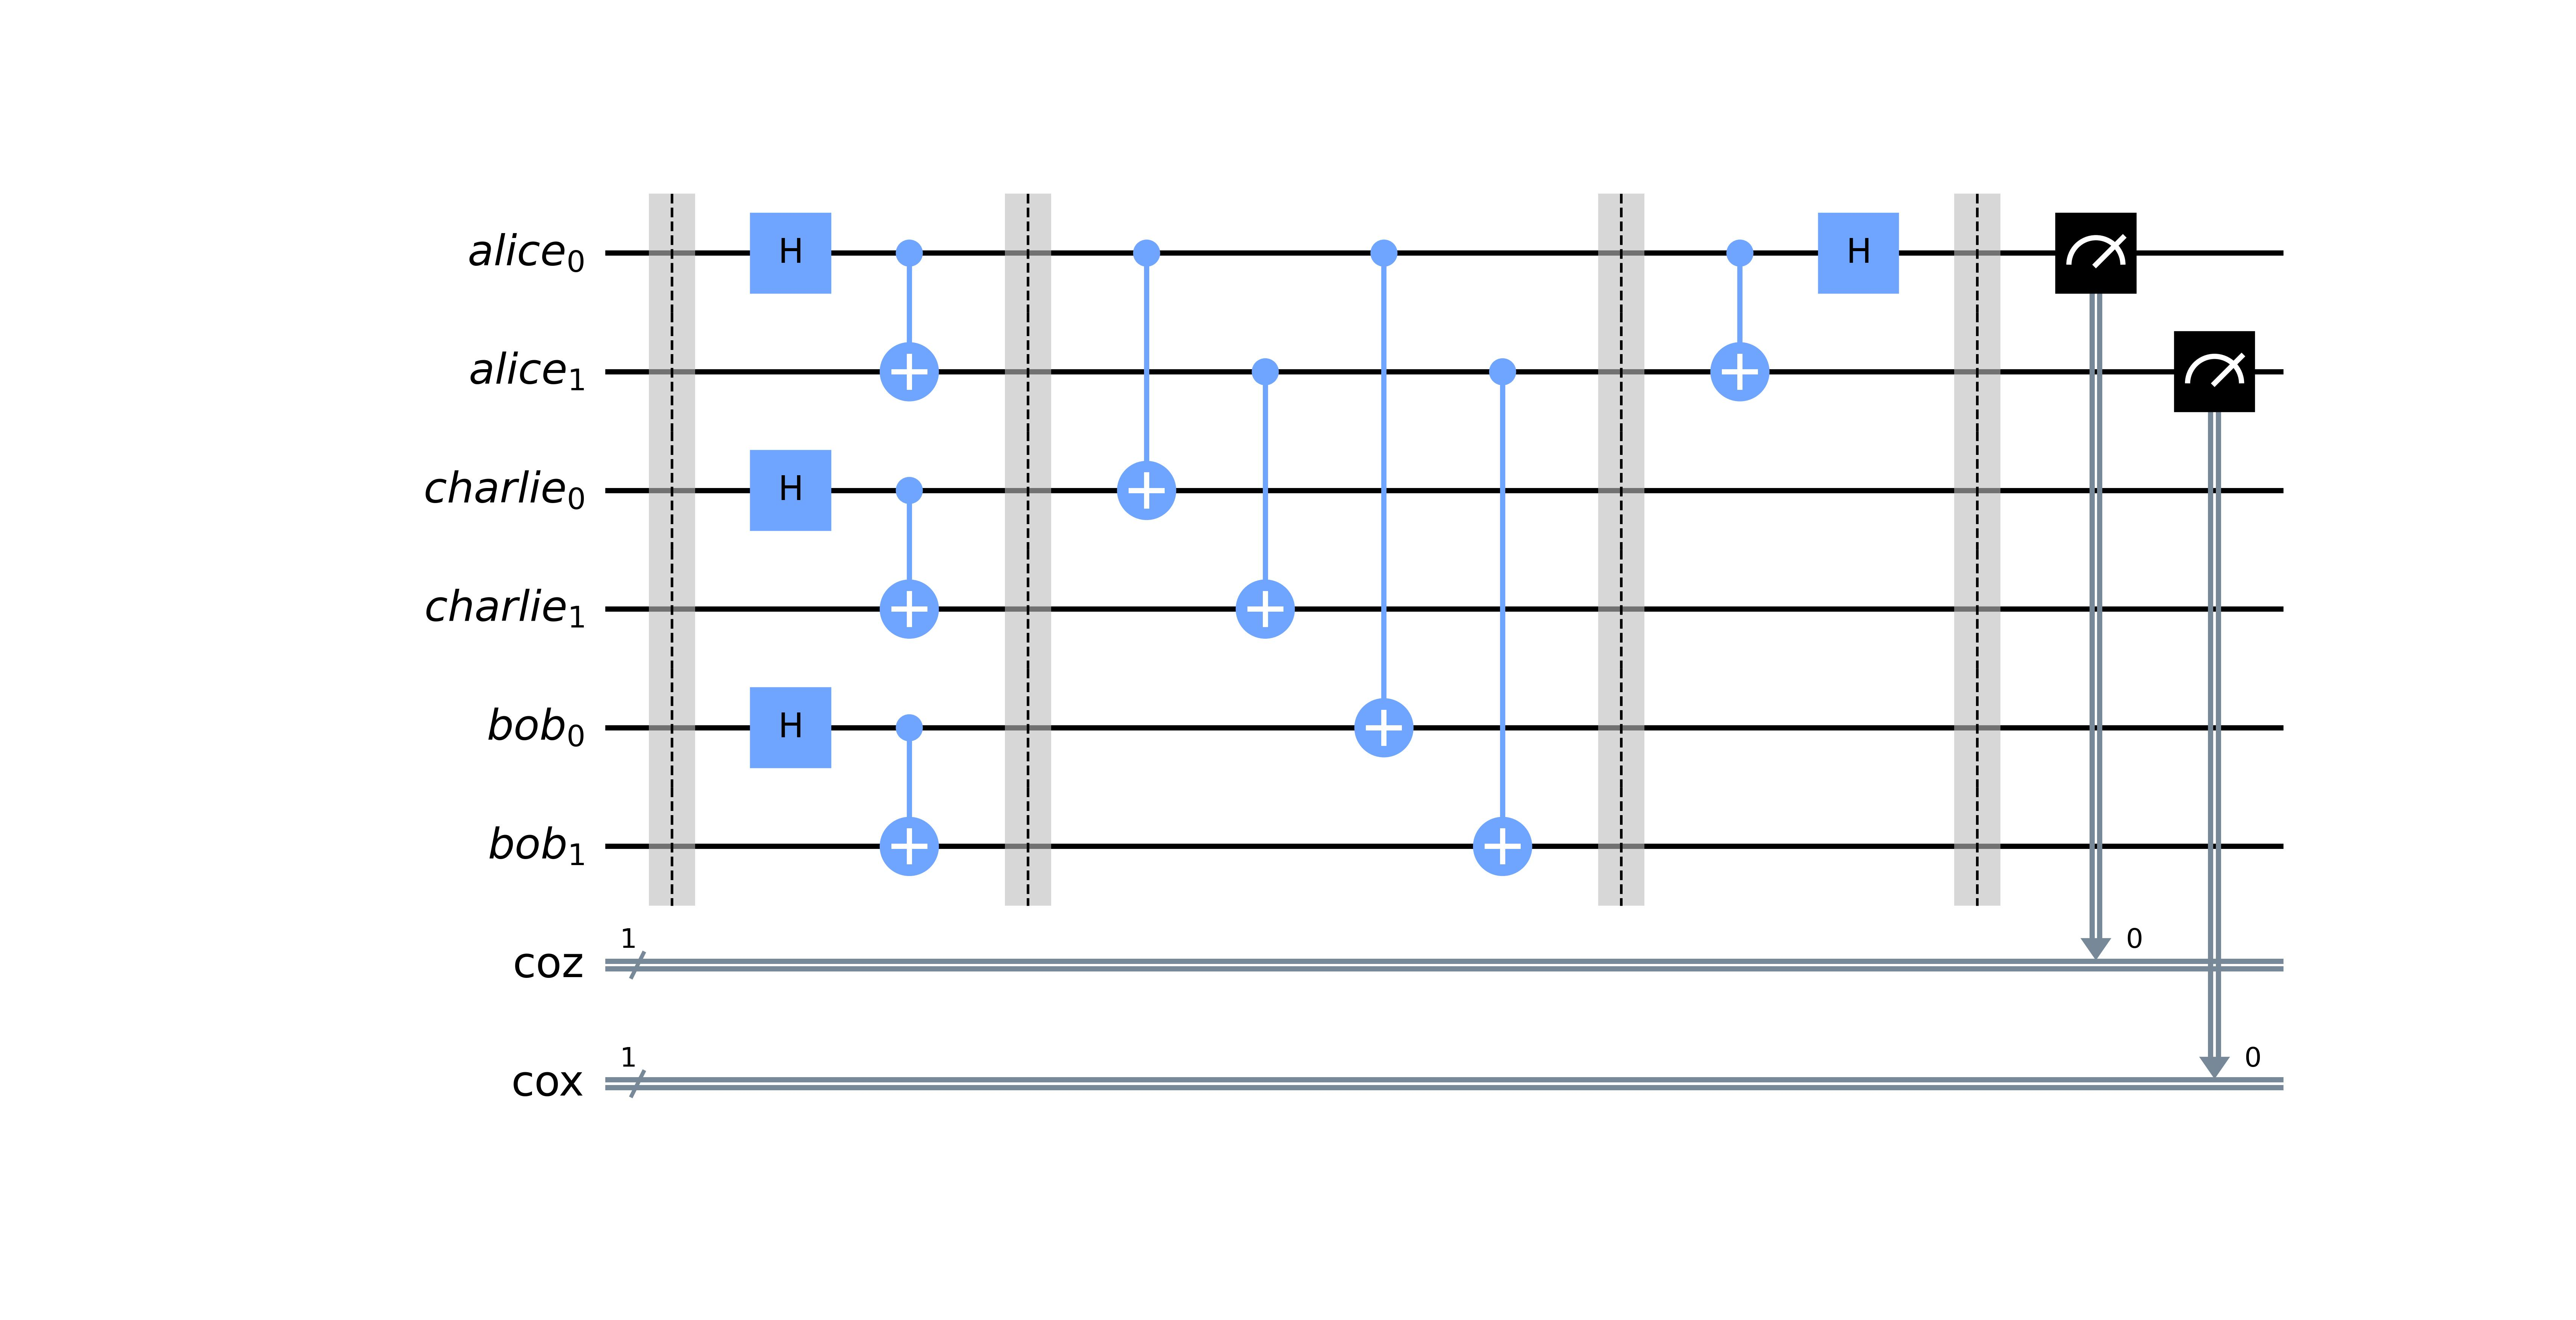
\includegraphics[width=\linewidth]{figures/purification_bennett.jpg}
    \caption[Bennett's purification protocol circuit]{Quantum circuit for Bennett's purification protocol}
    \label{fig:purification_bennett}
  \end{subfigure}
  \begin{subfigure}[b]{0.62\textwidth}
    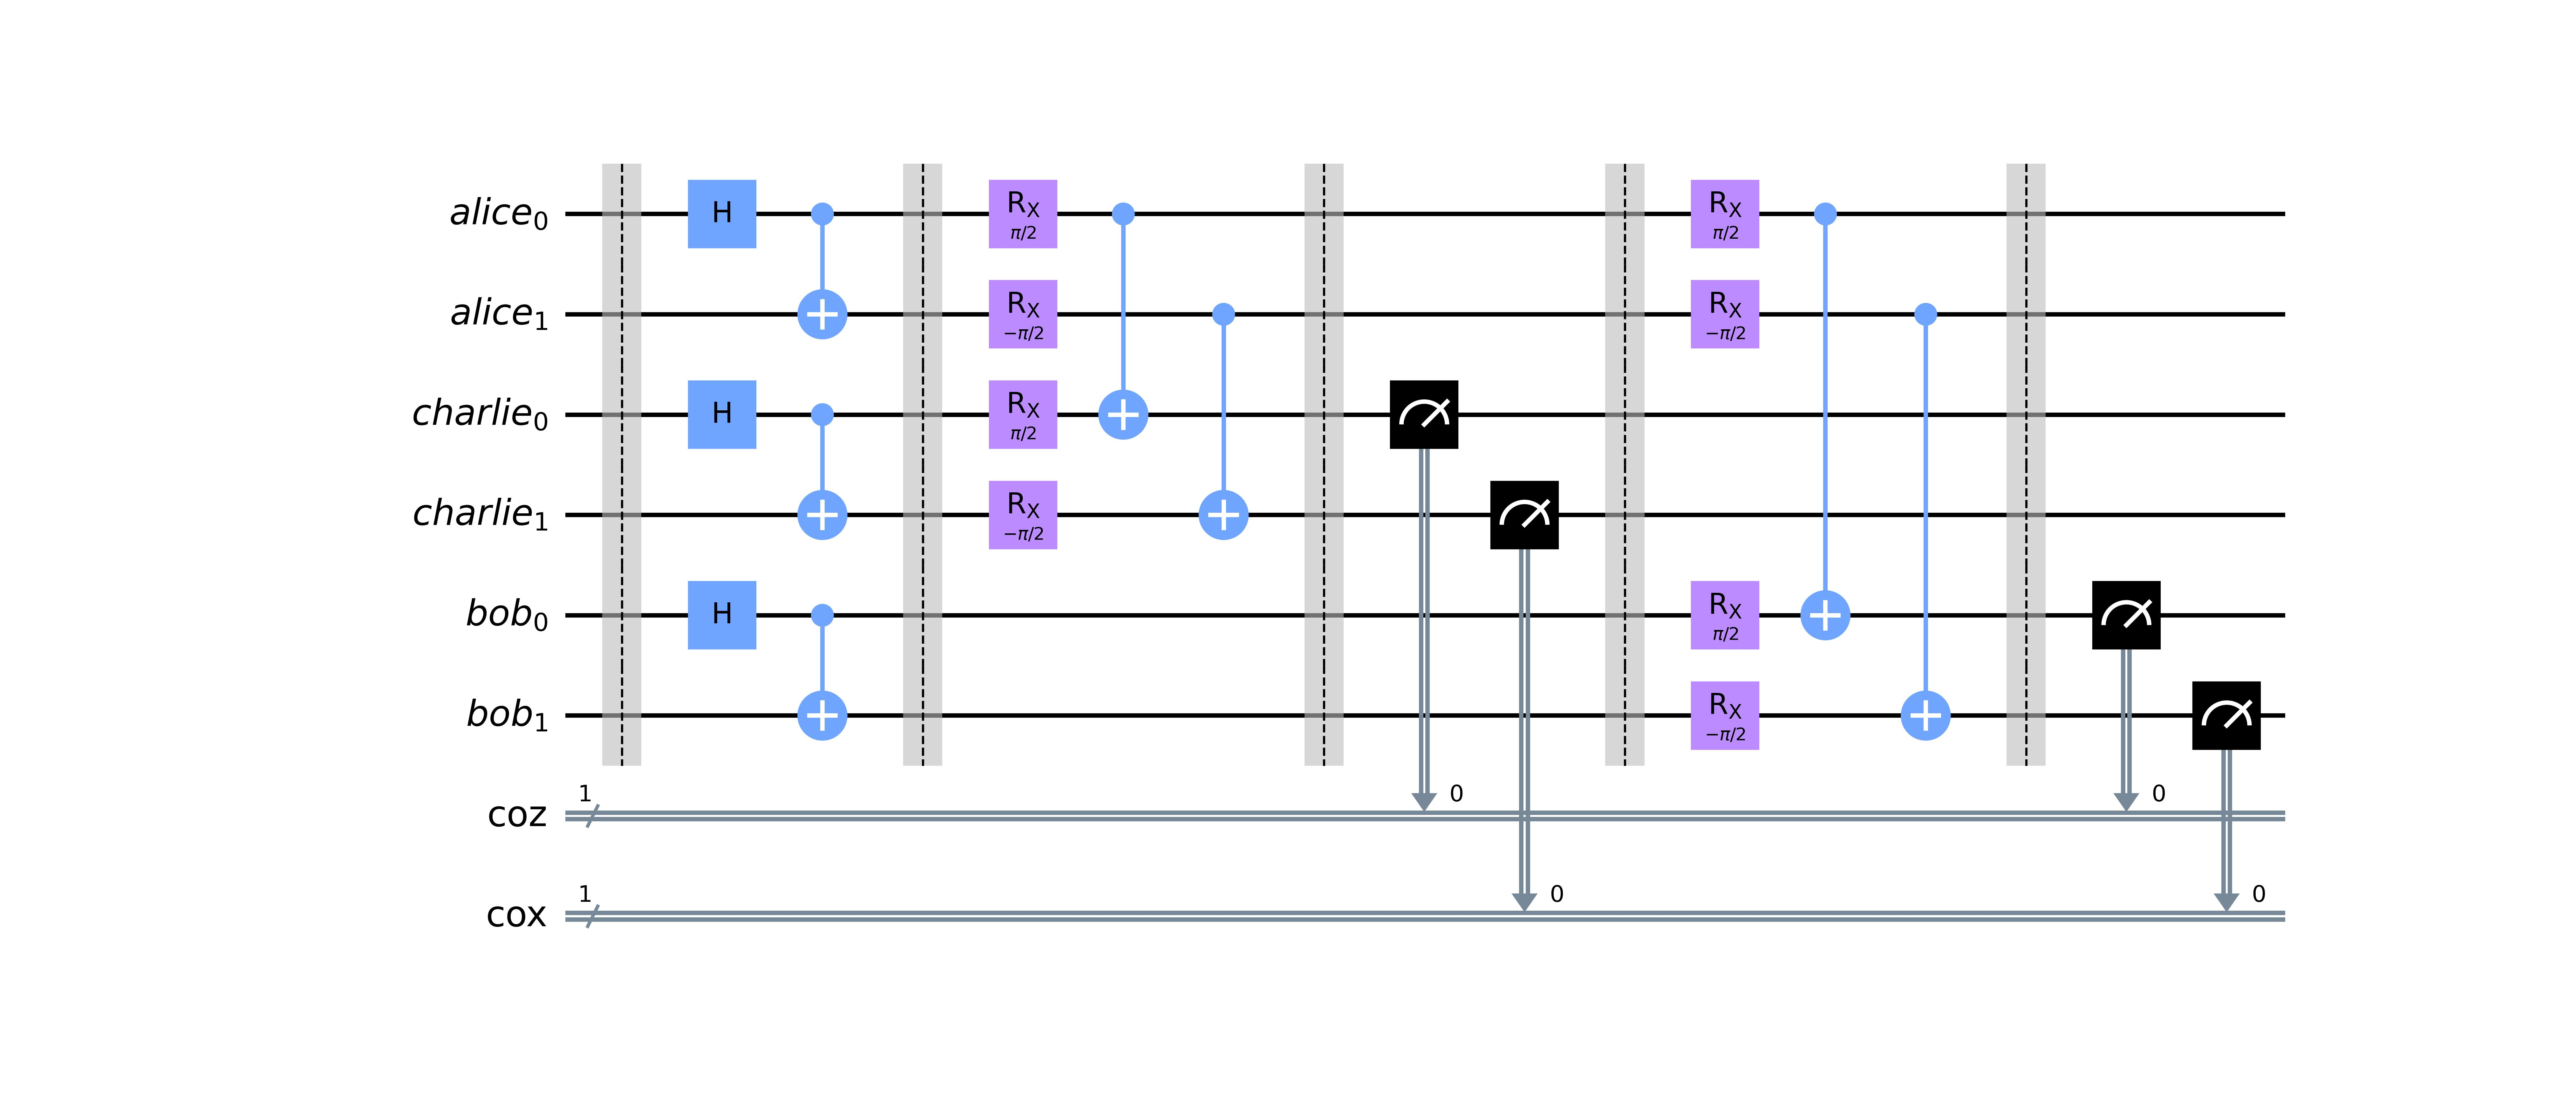
\includegraphics[width=\linewidth]{figures/purification_deutsch.jpg}
    \caption[Deutsch's purification protocol circuit]{Quantum circuit for Deutsch's purification protocol}
    \label{fig:purification_deutsch}
  \end{subfigure}
  \caption[Purification protocols]{Circuit implementation of the Deutsch's and Bennett's purification protocols.}
  \label{fig:sdfg}
\end{figure}

\subsection{Quantum Entanglement Swapping}
The quantum entanglement swapping circuit has a construction approach similar to the teleportation protocol. Here, we demonstrated the teleportation of an entangled qubit by entangling one qubit of Alice's Bell pair with another qubit of Bob's Bell pair. This is significant because it allows for states previously not entangled and which had never interacted with each other before to become entangled with each other. This is the guiding principle to extending the length of a quantum link.

The elementary construction of the entanglement swapping circuit contains two Bell pairs which together form a combined 4-qubit quantum state $|\psi\rangle_{ABCD} = |\Phi^{+}\rangle_{AB} \otimes |\Phi^{+}\rangle_{CD}$. (Bell-state measurement) BSM measurement is performed between the qubits in B and C. Depending on the results of the measurement, an appropriate Pauli correction operation {\textit{I, Z, X, Y}} gets performed on the qubit in D \cite{Das_2021}. The result is the projection of qubits in A and D into the state $|\Phi^{+}\rangle_{AD}$ and the entanglement between nodes B and C in the state $|\Phi^{+}\rangle_{BC}$. Teleportation can now occur directly from node A to D because the entanglement distributed to D from A maintains a complete quantum communication link not limited by spatial separation.
\begin{figure}[ht]
    \centering
    
\includegraphics[width=0.90\textwidth]{figures/entanglement_swapping.jpg}
    \caption[Entanglement swapping protocol circuit]{Quantum circuit for quantum entanglement swapping protocol}
    \label{fig:entanglement_swapping}
\end{figure}
Having executed the circuit in Figure \ref{fig:entanglement_swapping} in the QASM simulator, the measurement results gotten were as in Figure \ref{fig:entanglement_swapping_verification}. As expected, Alice's entangled qubit $alice_0$, when measured is in the state $|0\rangle$ with near $100\%$ probability together with Bob's other qubit $bob_1$ with whom they are entangled. This results act as proof of a successful entanglement swapping protocol.
\begin{figure}[ht]
    \centering
    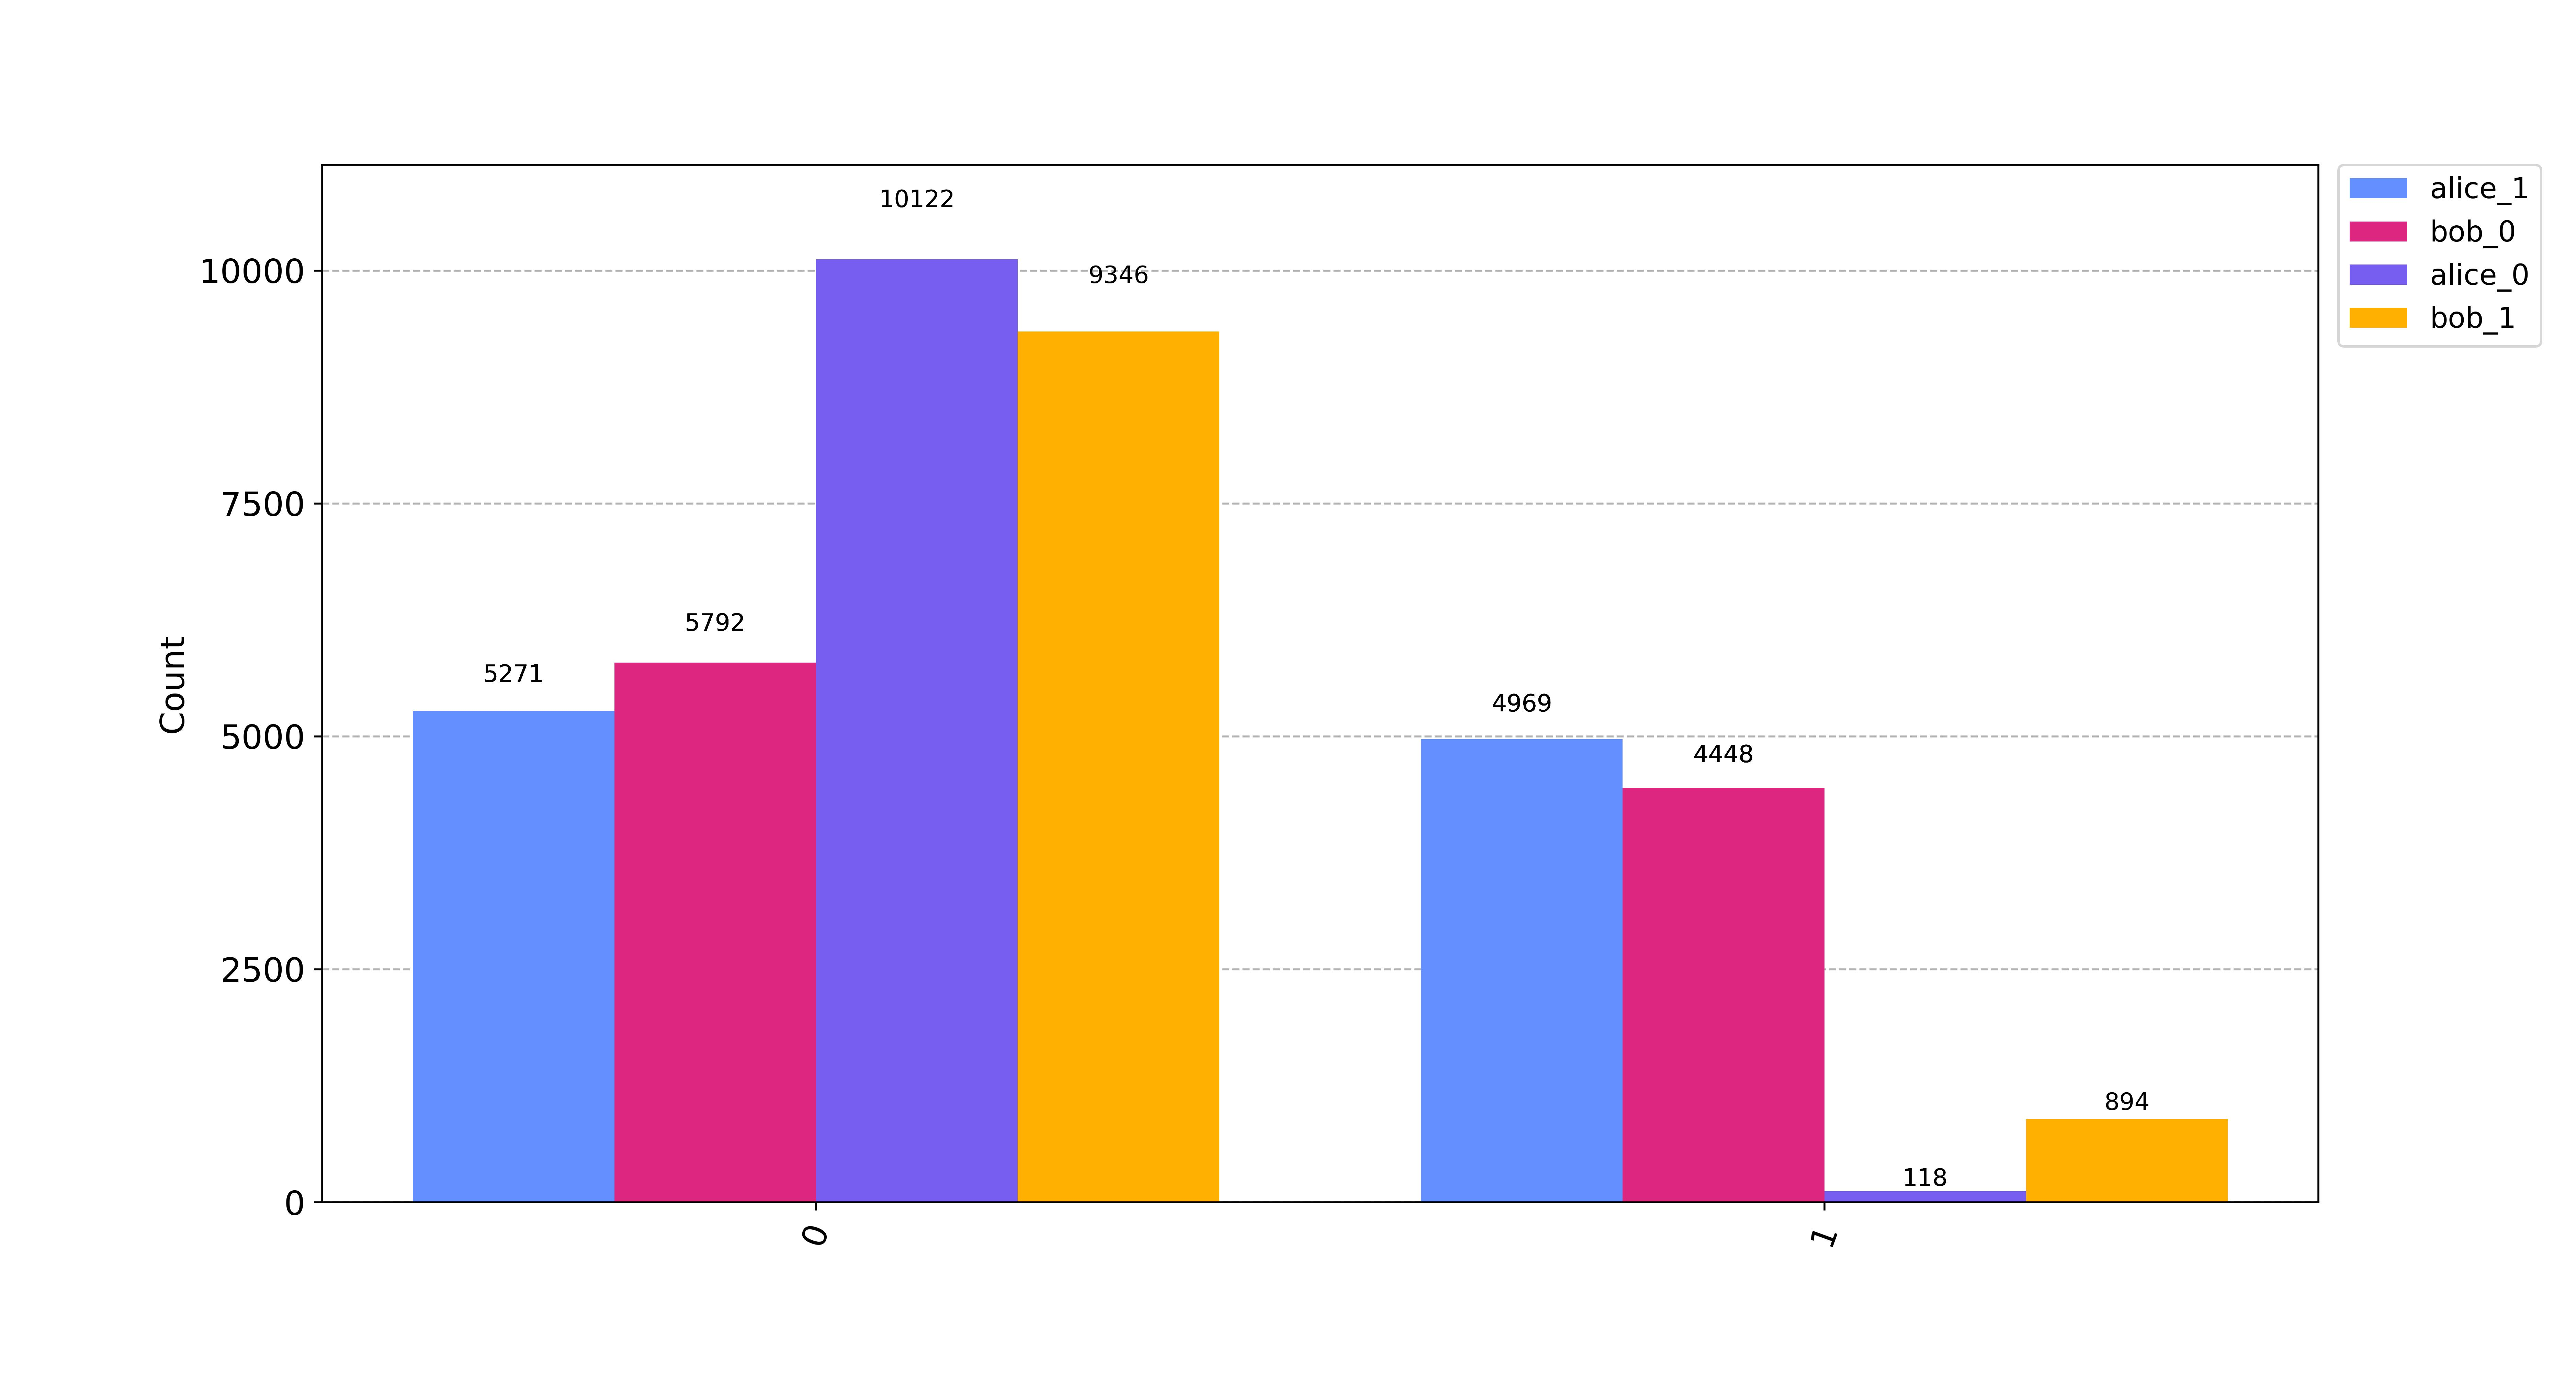
\includegraphics[width=0.5\textwidth]{figures/entanglement_swapping_verification.jpg}
    \caption[Entanglement swapping verification results]{Results for the verification of quantum entanglement swapping}
    \label{fig:entanglement_swapping_verification}
\end{figure}
%%%%%%%%%%%%%%%%%%%%%%%%%%%%%%%%%%%%%%%%%%%%%%%%%%%%%%%%%%%%%%
%%%%%%%%%%%%%%%%%%%%%%%%%%%%%%%%%%%%%%%%%%%%%%%%%%%%%%%%%%%%%%
\section{Results and Discussion}
\subsection{Complete Quantum Repeater Architecture}
Combining all the necessary components, we arrived at a complete implementation of a quantum repeater and its augmenting components in a quantum network. The circuit architecture is as in Figure \ref{fig:quantum_repeater_deutsch} and Figure \ref{fig:quantum_repeater_bennett}.

Alice's and Bob's Bell pairs are first generated. One qubit from each Bell pair gets transmitted to Alice and Bob through a classical channel. The remaining qubits from each Bell pair get transmitted through a classical channel to quantum memory devices found on the quantum repeater. The transmission of these qubits is emulated using SWAP gates. Through heralding, a classical message is sent to the repeater indicating that Alice's and Bob's qubits are ready for swapping. The heralding helps to synchronize the swapping protocol. The qubits in the quantum memory devices get transmitted to their respective quantum channels, ready for swapping. This transmission is again represented by SWAP gates.
\begin{figure}[ht]
    \centering
    \includegraphics[width=\textwidth]{figures/quantum_repeater_deutsch.jpg}
    \caption[Complete quantum repeater using Deutsch's purification protocol]{Quantum circuit for the full complete quantum repeater, implementing Deutsch's purification protocol just before the swapping protocol stage. $qgen\_alice$ and $qgen\_bob$ represents the modules generating Alice's and Bob's entangled qubits respectively. $qmem$ represents quantum memory devices present in a quantum repeater. The transmission of qubits through classical channels to either quantum channels of quantum memory is emulated using SWAP gates.}
    \label{fig:quantum_repeater_deutsch}
\end{figure}
\begin{figure}[ht]
    \centering
    \includegraphics[width=\textwidth]{figures/quantum_repeater_bennett.jpg}
    \caption[Complete quantum repeater using Bennett's purification protocol]{Quantum circuit for the full complete quantum repeater, implementing Bennett's purification protocol just before the swapping protocol stage.}
    \label{fig:quantum_repeater_bennett}
\end{figure}
In this circuit in Figure \ref{fig:quantum_repeater_deutsch}, Deutsch's purification protocol is done just before swapping. Thereafter entanglement swapping protocol is done. Finally, Alice's and Bob's qubits are measured out in the Bell basis.

The presented circuit architecture provides a real-world implementation of the quantum repeater protocol. We used it to investigate our remaining objectives regarding purification strategies and optimization schemes.
% The circuit architecture demonstrates the quantum repeater protocol as it is to be implemented in the real world upon deployment. Using this quantum repeater circuit, we moved to investigate our remaining objectives regarding purification strategies and optimization schemes.

\subsection{Purification Strategy}
%[A number of] experimental simulations were carried out to determine the optimum purification strategy.
Identifying an optimum purification strategy for near-term quantum repeaters means better efficiency of operation of future practical quantum repeaters. In total, four purification strategies were used in the simulations. The strategies differ in the stages at which they apply the purification protocol.

The stages are: Bell-pair production stage, entanglement swapping protocol stage and readout stage. The variations of those stages inspired the four purification strategies:
\begin{itemize}
    \item Post Bell-pair production purification strategy. Performs purification after Bell-pairs are created.
    \item Post swap purification strategy. Performs purification after every entanglement swapping protocol.
    \item Repeated post swap purification strategy. Performs several purification instances successively after every entanglement swapping protocol. In our simulations, we set our number of instances to two.
    \item Pre and post swap purification strategy. Performs purification in an alternating manner, that is before and after an entanglement swapping protocol.
\end{itemize}
% post Bell-pair production purification strategy, post swap purification strategy, repeated post swap purification strategy and pre and post swap purification strategy.
%purification after Bell-pairs are created, purification after every swap, entanglement swapping alternating purification that is, before and after swapping, repeated purification after every swap.
%and a custom purification strategy aiming at a suitable combination of various steps.

The experimental simulations were only conducted using Deutsch's purification protocol. This was based on the assumption that the results would be similar with any other purification protocol since only the stage at which purification was conducted was being varied.

Qiskit provides a noise model module that we used to create the a simplified approximate noise model based on the properties of real quantum computer devices. The errors due to the noise model are sufficient to emulate real world errors.

To conduct the purification strategy simulations, a compact form of the circuit in Figure \ref{fig:quantum_repeater_deutsch} was used. An initializer instruction was appended at the beginning of the circuit to perform a reset on Alice's qubit, setting it into the state $|0\rangle$ then applying gates to turn it into a random state $|\psi\rangle$. After the initialization instruction followed the quantum repeater protocol after which an inverse initialization instruction was appended. The inverse initialization instruction works to revert the random state $|\psi\rangle$ back to the state $|0\rangle$. Thus, upon measurement on Alice's and Bob's qubits at the end, ideally, one should get the state $|00\rangle$.
\begin{figure}[ht]
  \centering
  \begin{subfigure}[b]{0.45\textwidth}
    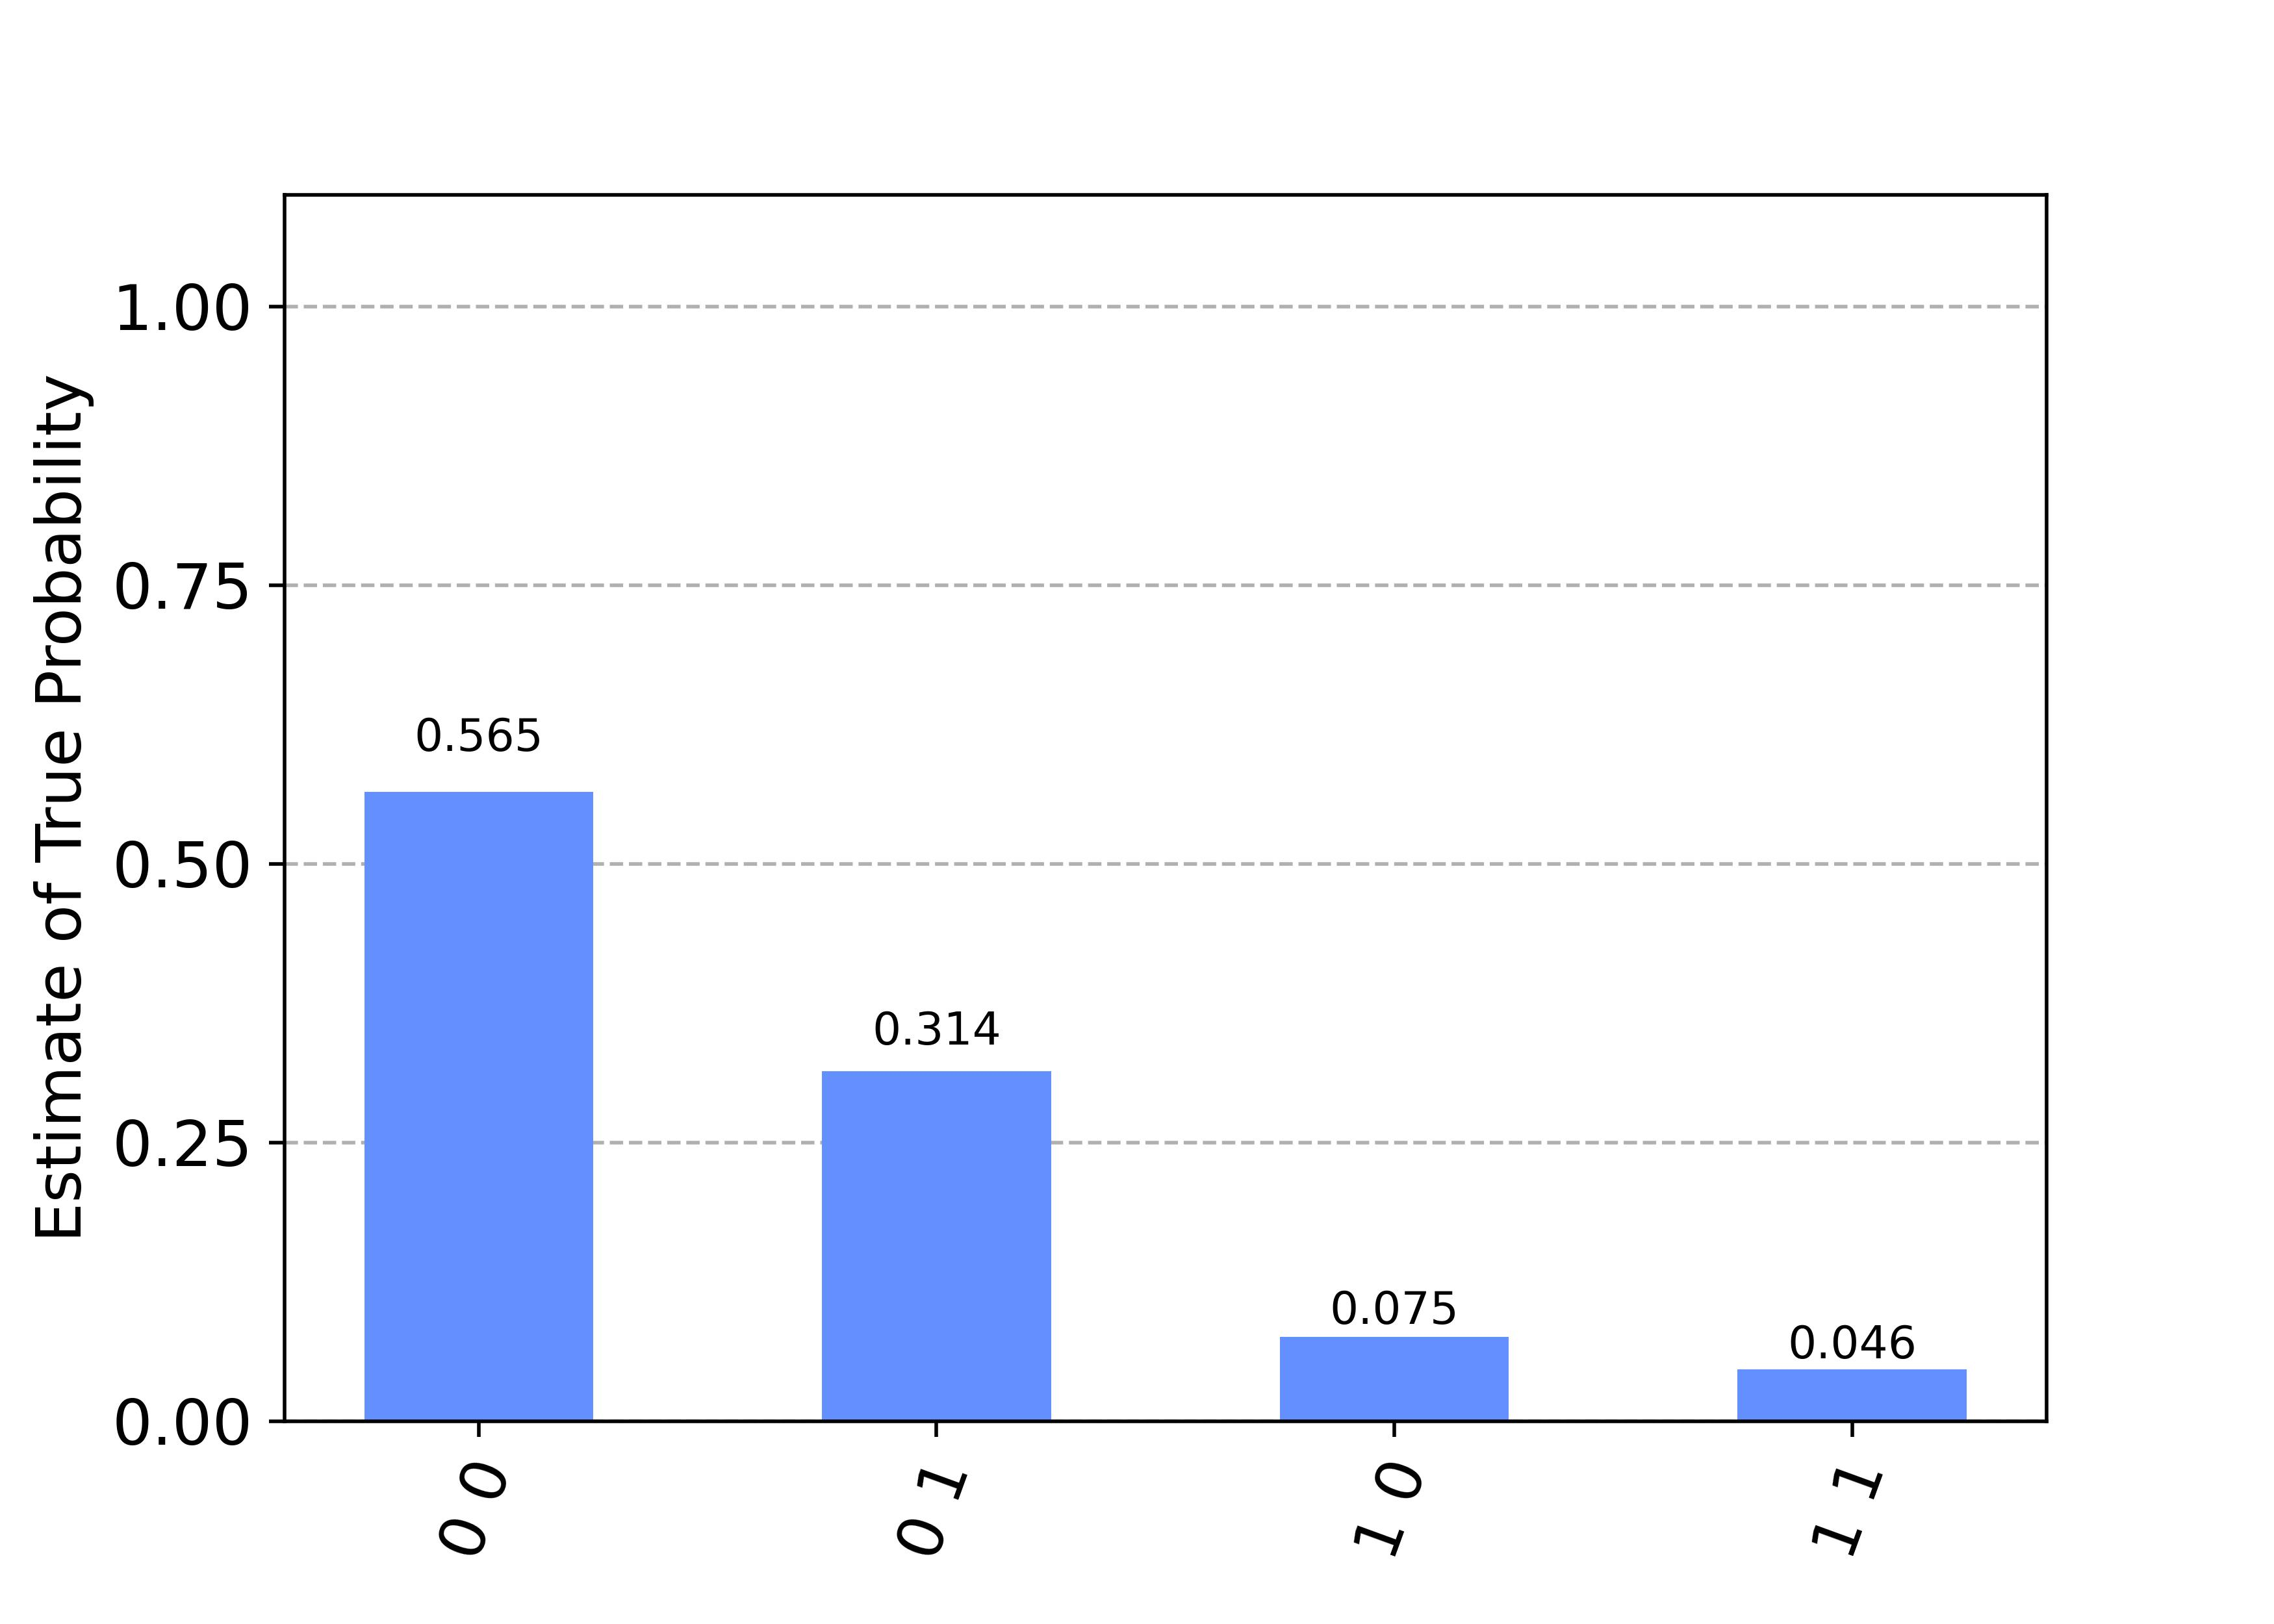
\includegraphics[width=\linewidth]{figures/dps_measurement_post_bell_pair.jpg}
    \caption{Post Bell-pair production purification strategy\\measurement results}
    \label{fig:image1}
  \end{subfigure}
  \begin{subfigure}[b]{0.45\textwidth}
    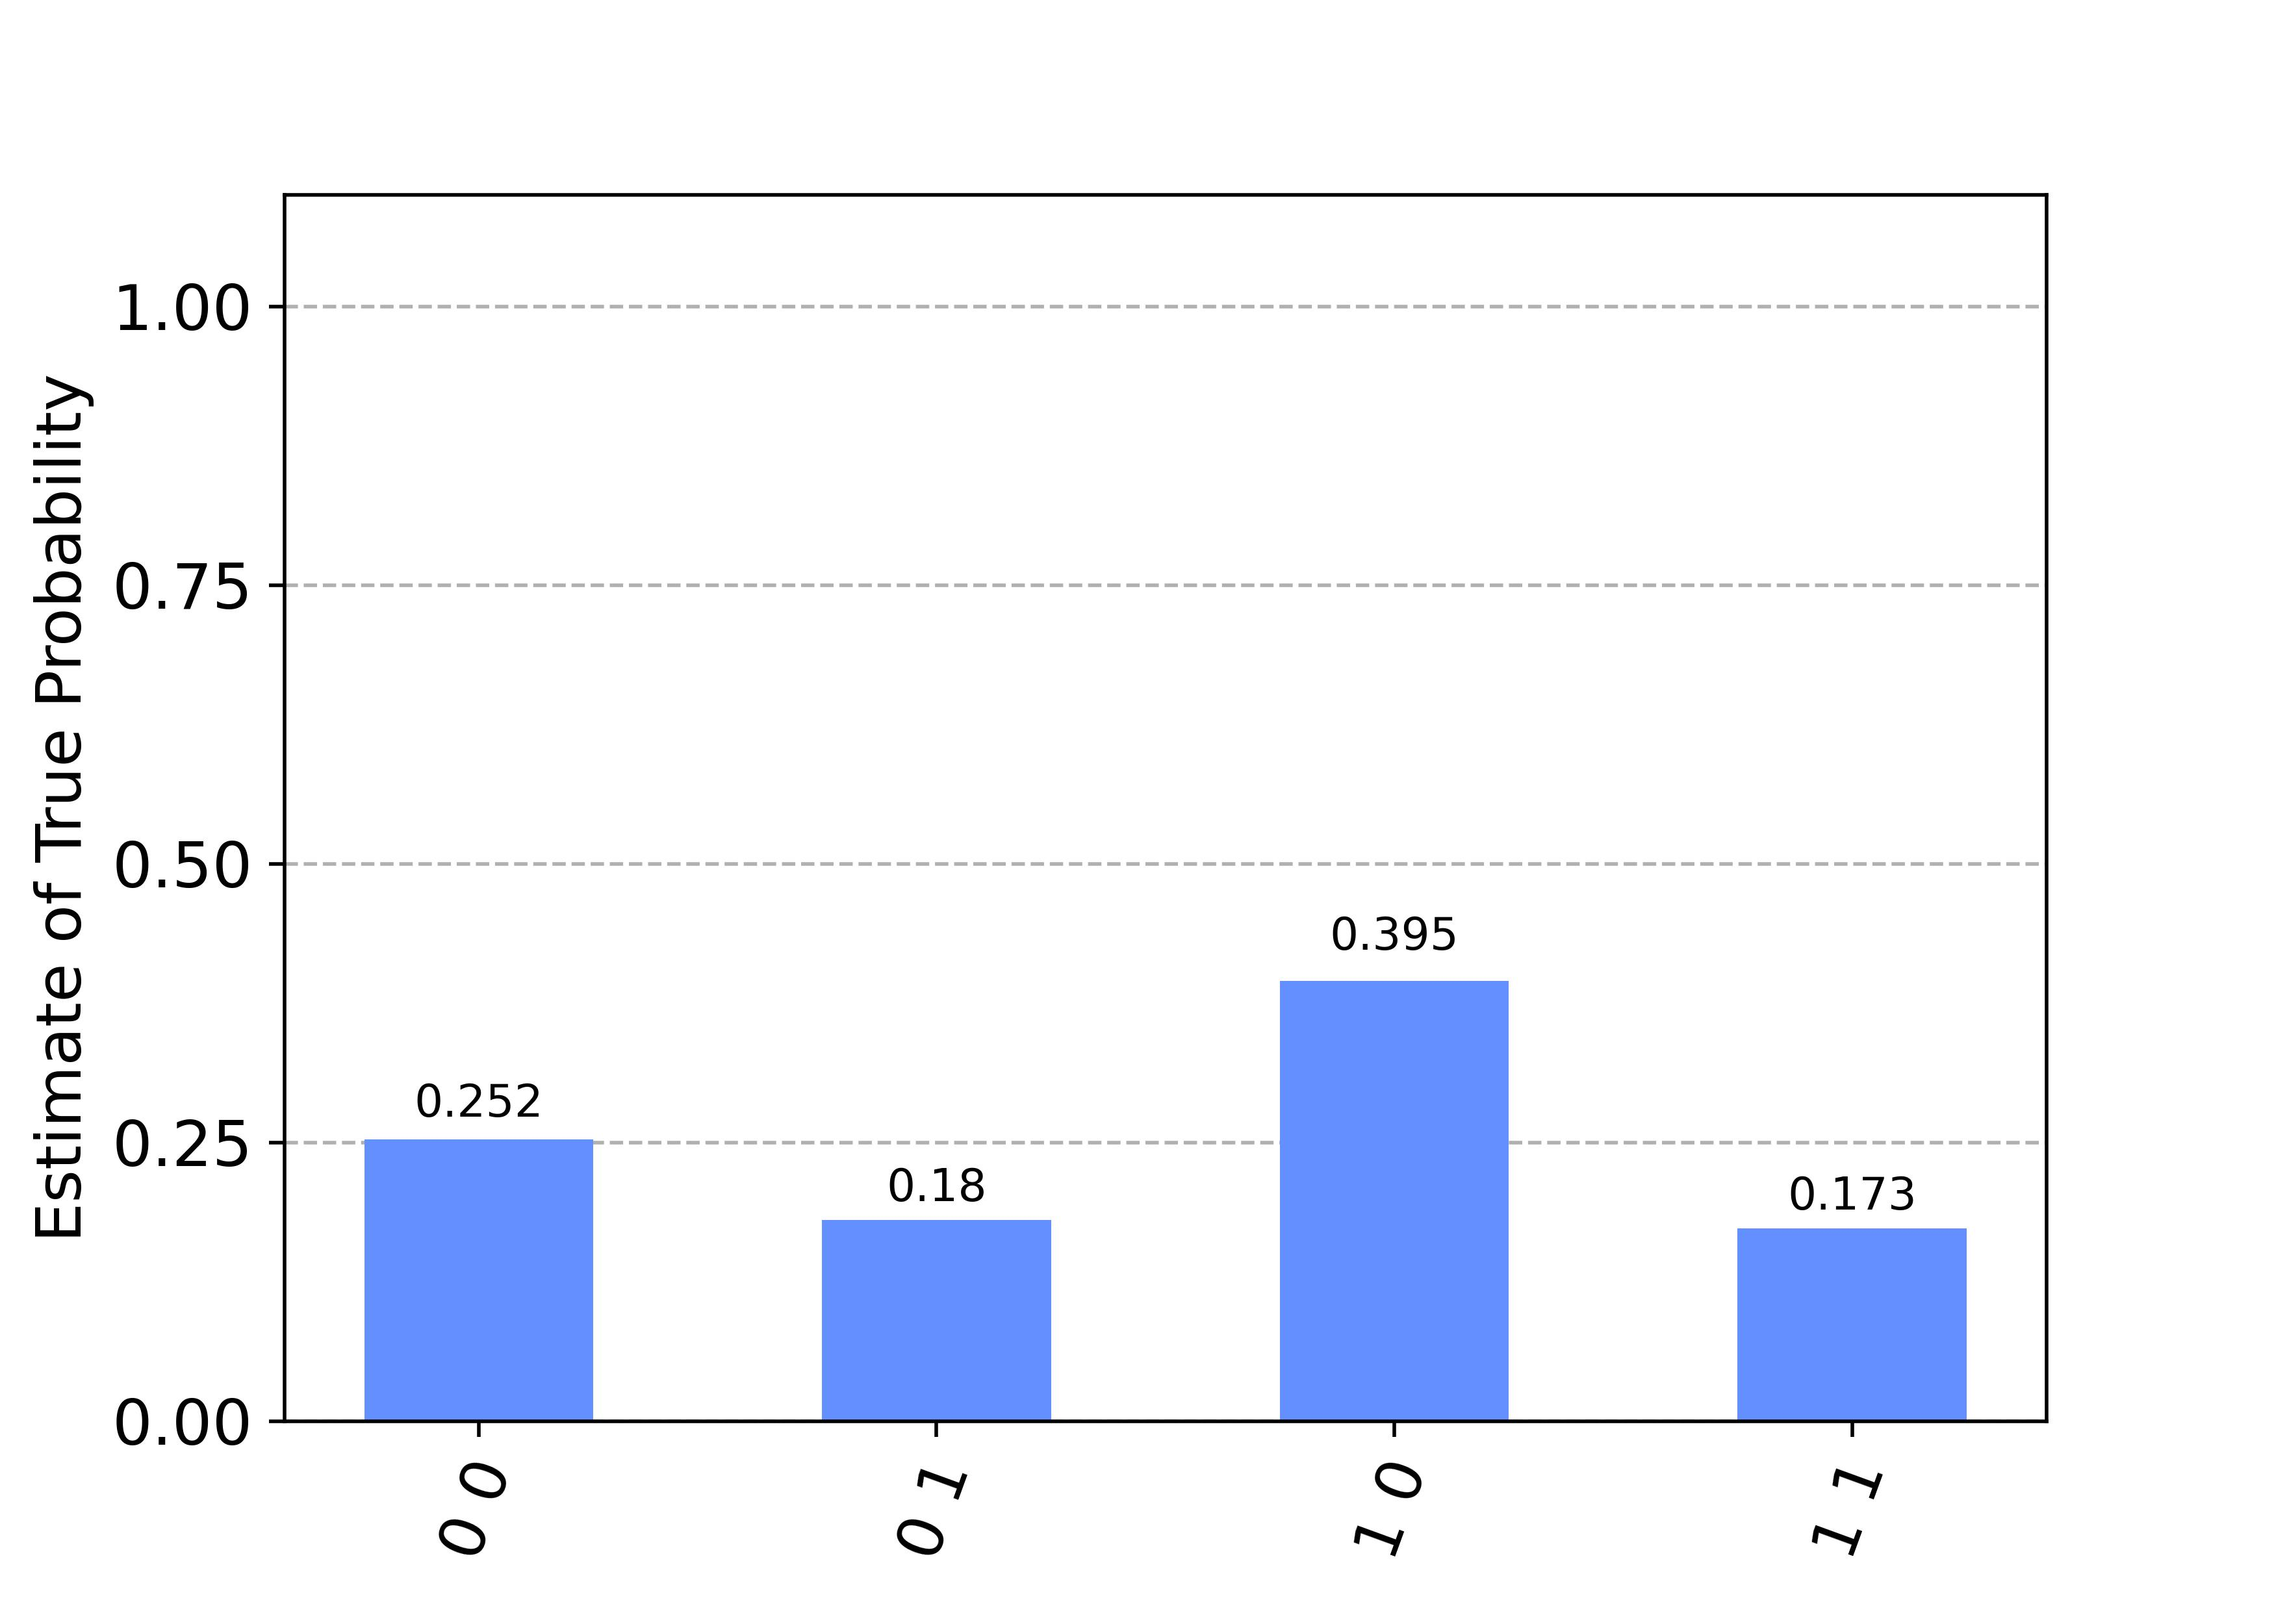
\includegraphics[width=\linewidth]{figures/dps_measurement_post_swap.jpg}
    \caption{Post swap purification strategy measurement results}
    \label{fig:image2}
  \end{subfigure}
  \\
  \begin{subfigure}[b]{0.45\textwidth}
    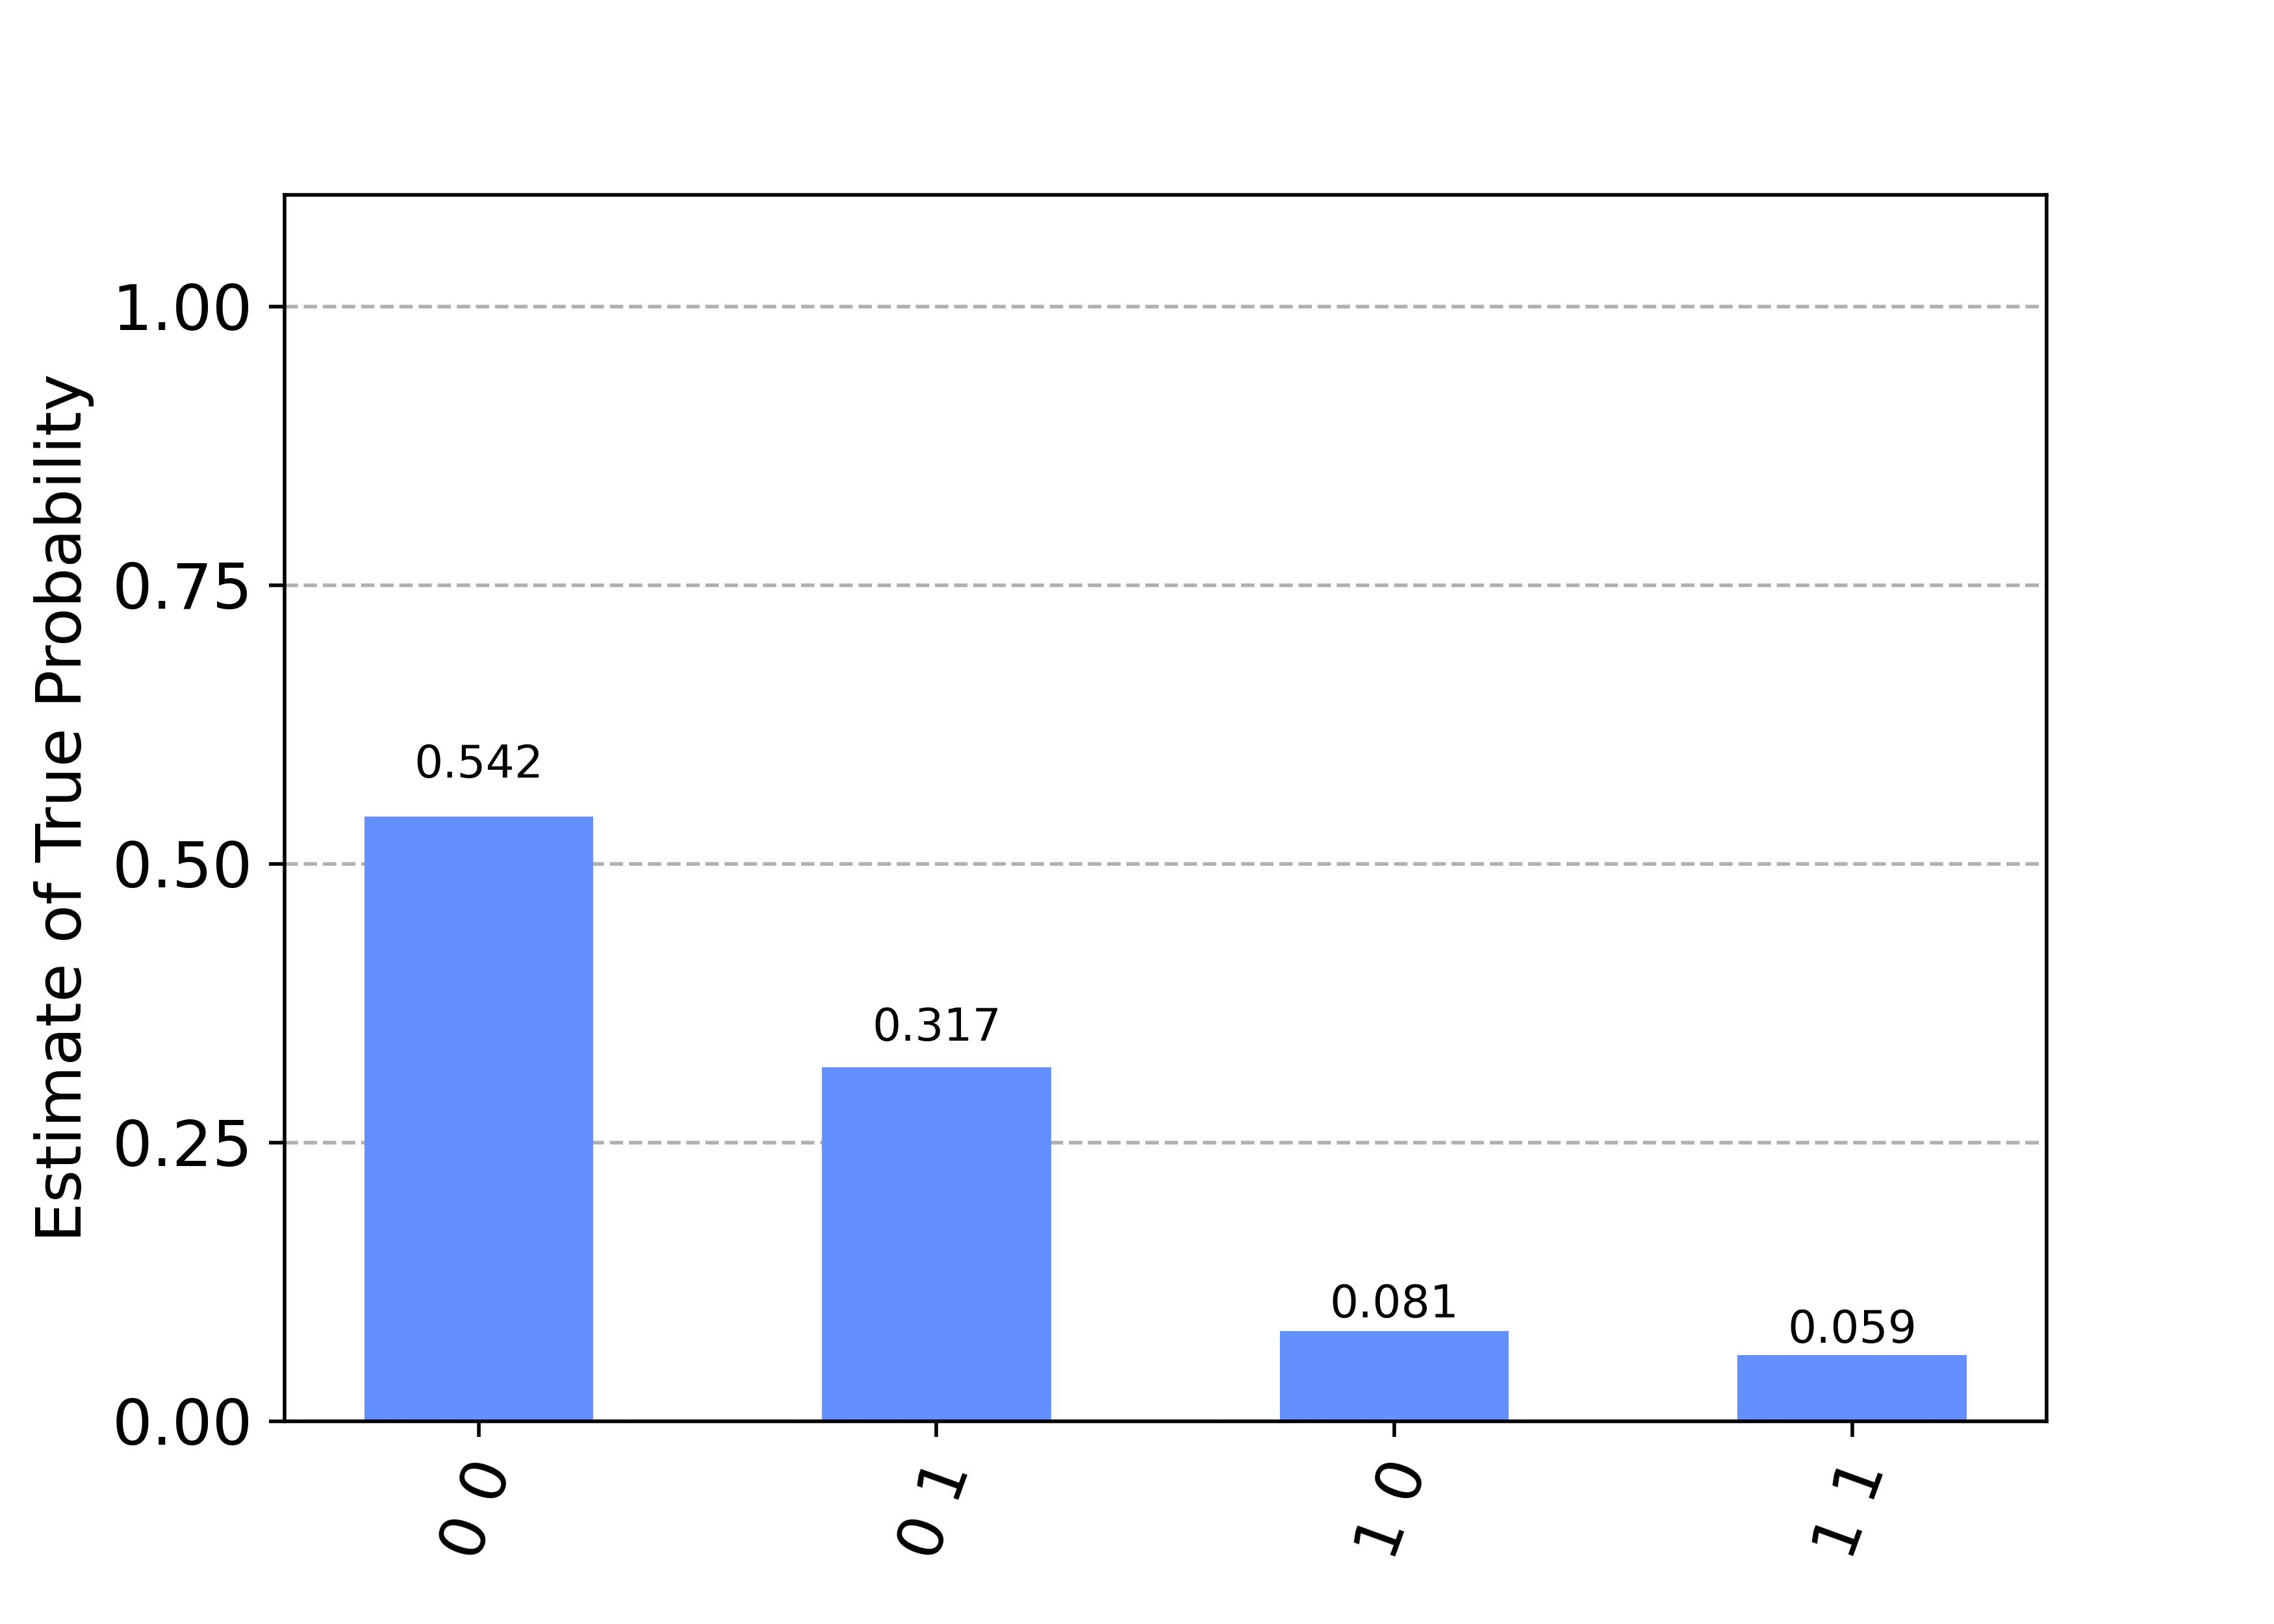
\includegraphics[width=\linewidth]{figures/dps_measurement_pre_and_post_swap.jpg}
    \caption{Pre-and-post swap purification strategy\\measurement results}
    \label{fig:image3}
  \end{subfigure}
  \begin{subfigure}[b]{0.45\textwidth}
    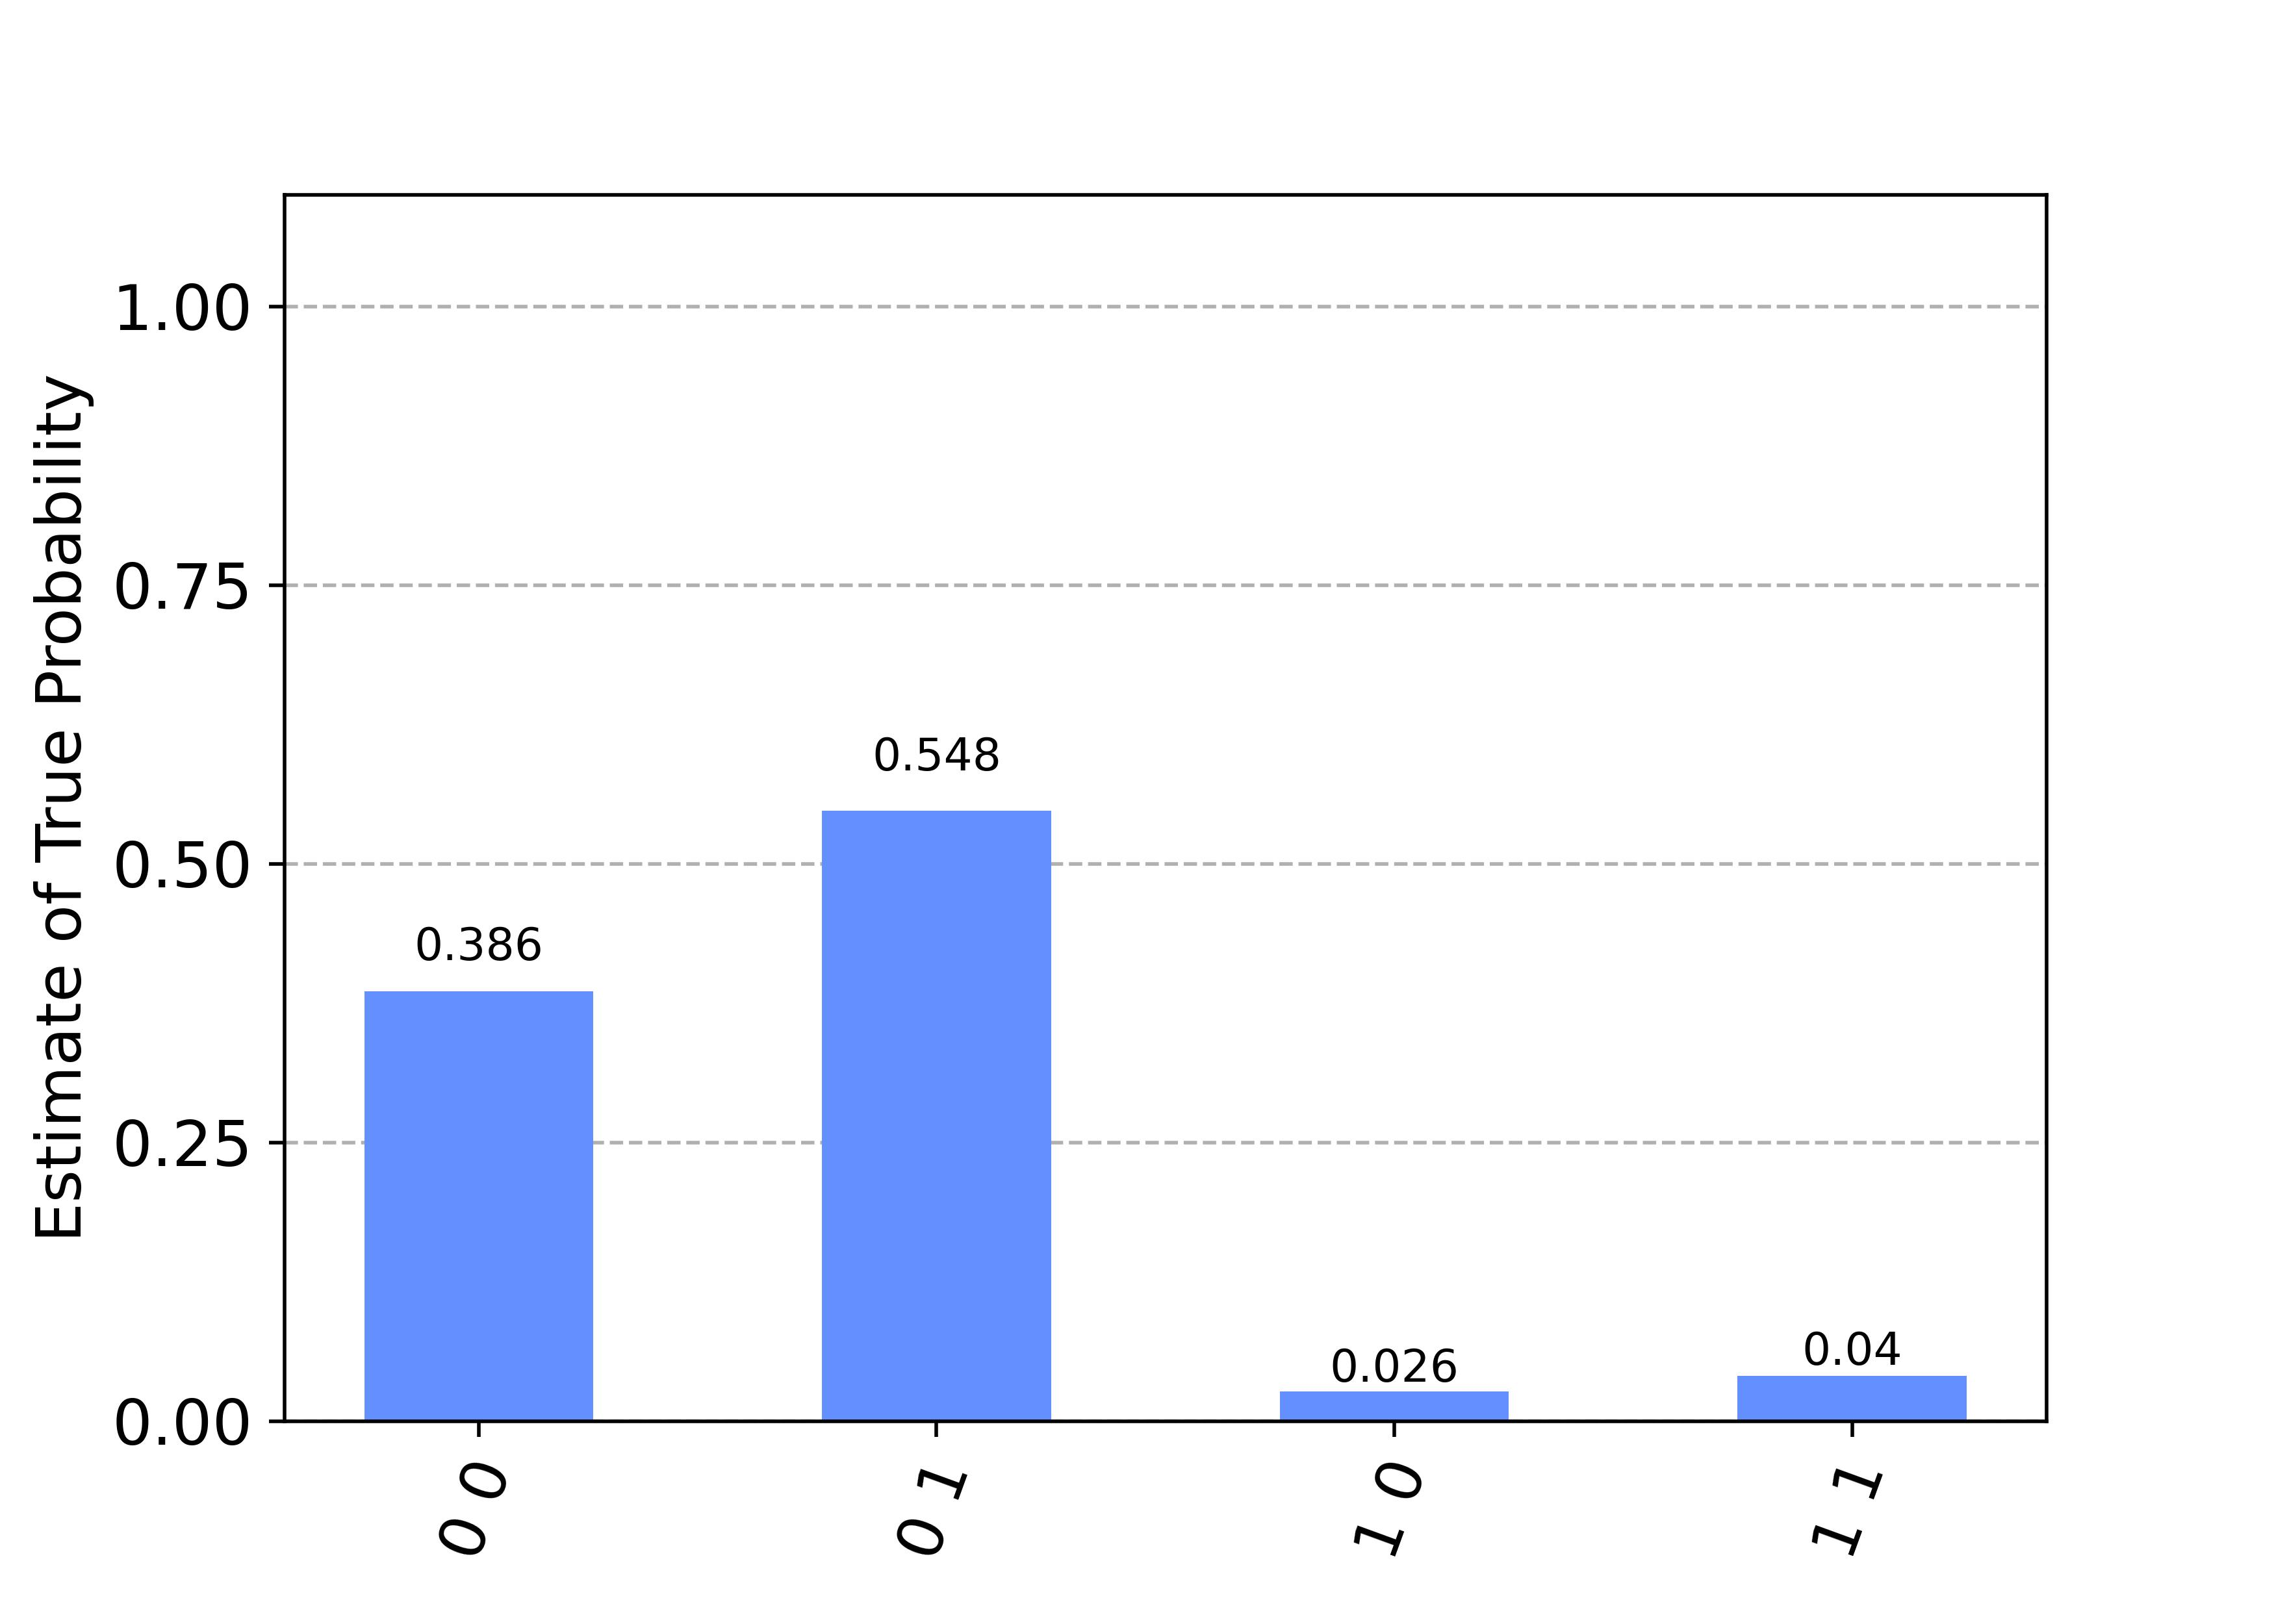
\includegraphics[width=\linewidth]{figures/dps_measurement_repeated_post_swap.jpg}
    \caption{Repeated post swap purification strategy measurement results}
    \label{fig:image4}
  \end{subfigure}
  \caption[Measurement results of the quantum Repeater protocol]{Measurement results of Alice's and Bob's qubits after a complete quantum repeater protocol.}
  \label{fig:deutsch_measurement_strategy_results}
\end{figure}
The entirety of the circuit was run 20 times, generating 20 independent measurement results each with its own set of probabilities for states $|00\rangle$, $|01\rangle$, $|10\rangle$ and $|11\rangle$. By averaging the results for all the 4 quantum states across all the 20 independent circuit runs, we got the following results as seen in Figure \ref{fig:deutsch_measurement_strategy_results}. The estimate of true probability converges to the true probability as we increase the number of circuit runs. In our case, 20 runs gave us sufficiently good results in reasonable simulation run time.

The results obtained were then used to verify that indeed one qubit from Alice's entangled qubit pair had been teleported to Bob. Measurement performed on either qubit can only yield state $|0\rangle$ or $|1\rangle$. The consequent plot is as seen in Figure \ref{fig:deutsch_purification_strategy_verification_results}. In the ideal case, we would have $100\%$ chance of measuring Bob's qubit in the state $|0\rangle$. Strategies that produced plots in Figure \ref{fig:deutsch_purification_strategy_verification_results_post_bell_pair}, Figure \ref{fig:deutsch_purification_strategy_verification_results_pre_post_swap} and Figure \ref{fig:deutsch_purification_strategy_verification_results_repeated_post_swap} have Bob's qubit being measured in the state $|0\rangle$ at estimated probabilities close to $100\%$. The higher estimated probabilities, indicate higher chances of the quantum repeater protocol having worked correctly as theoretically expected.

\begin{figure}[ht]
  \centering
  \begin{subfigure}[b]{0.45\textwidth}
    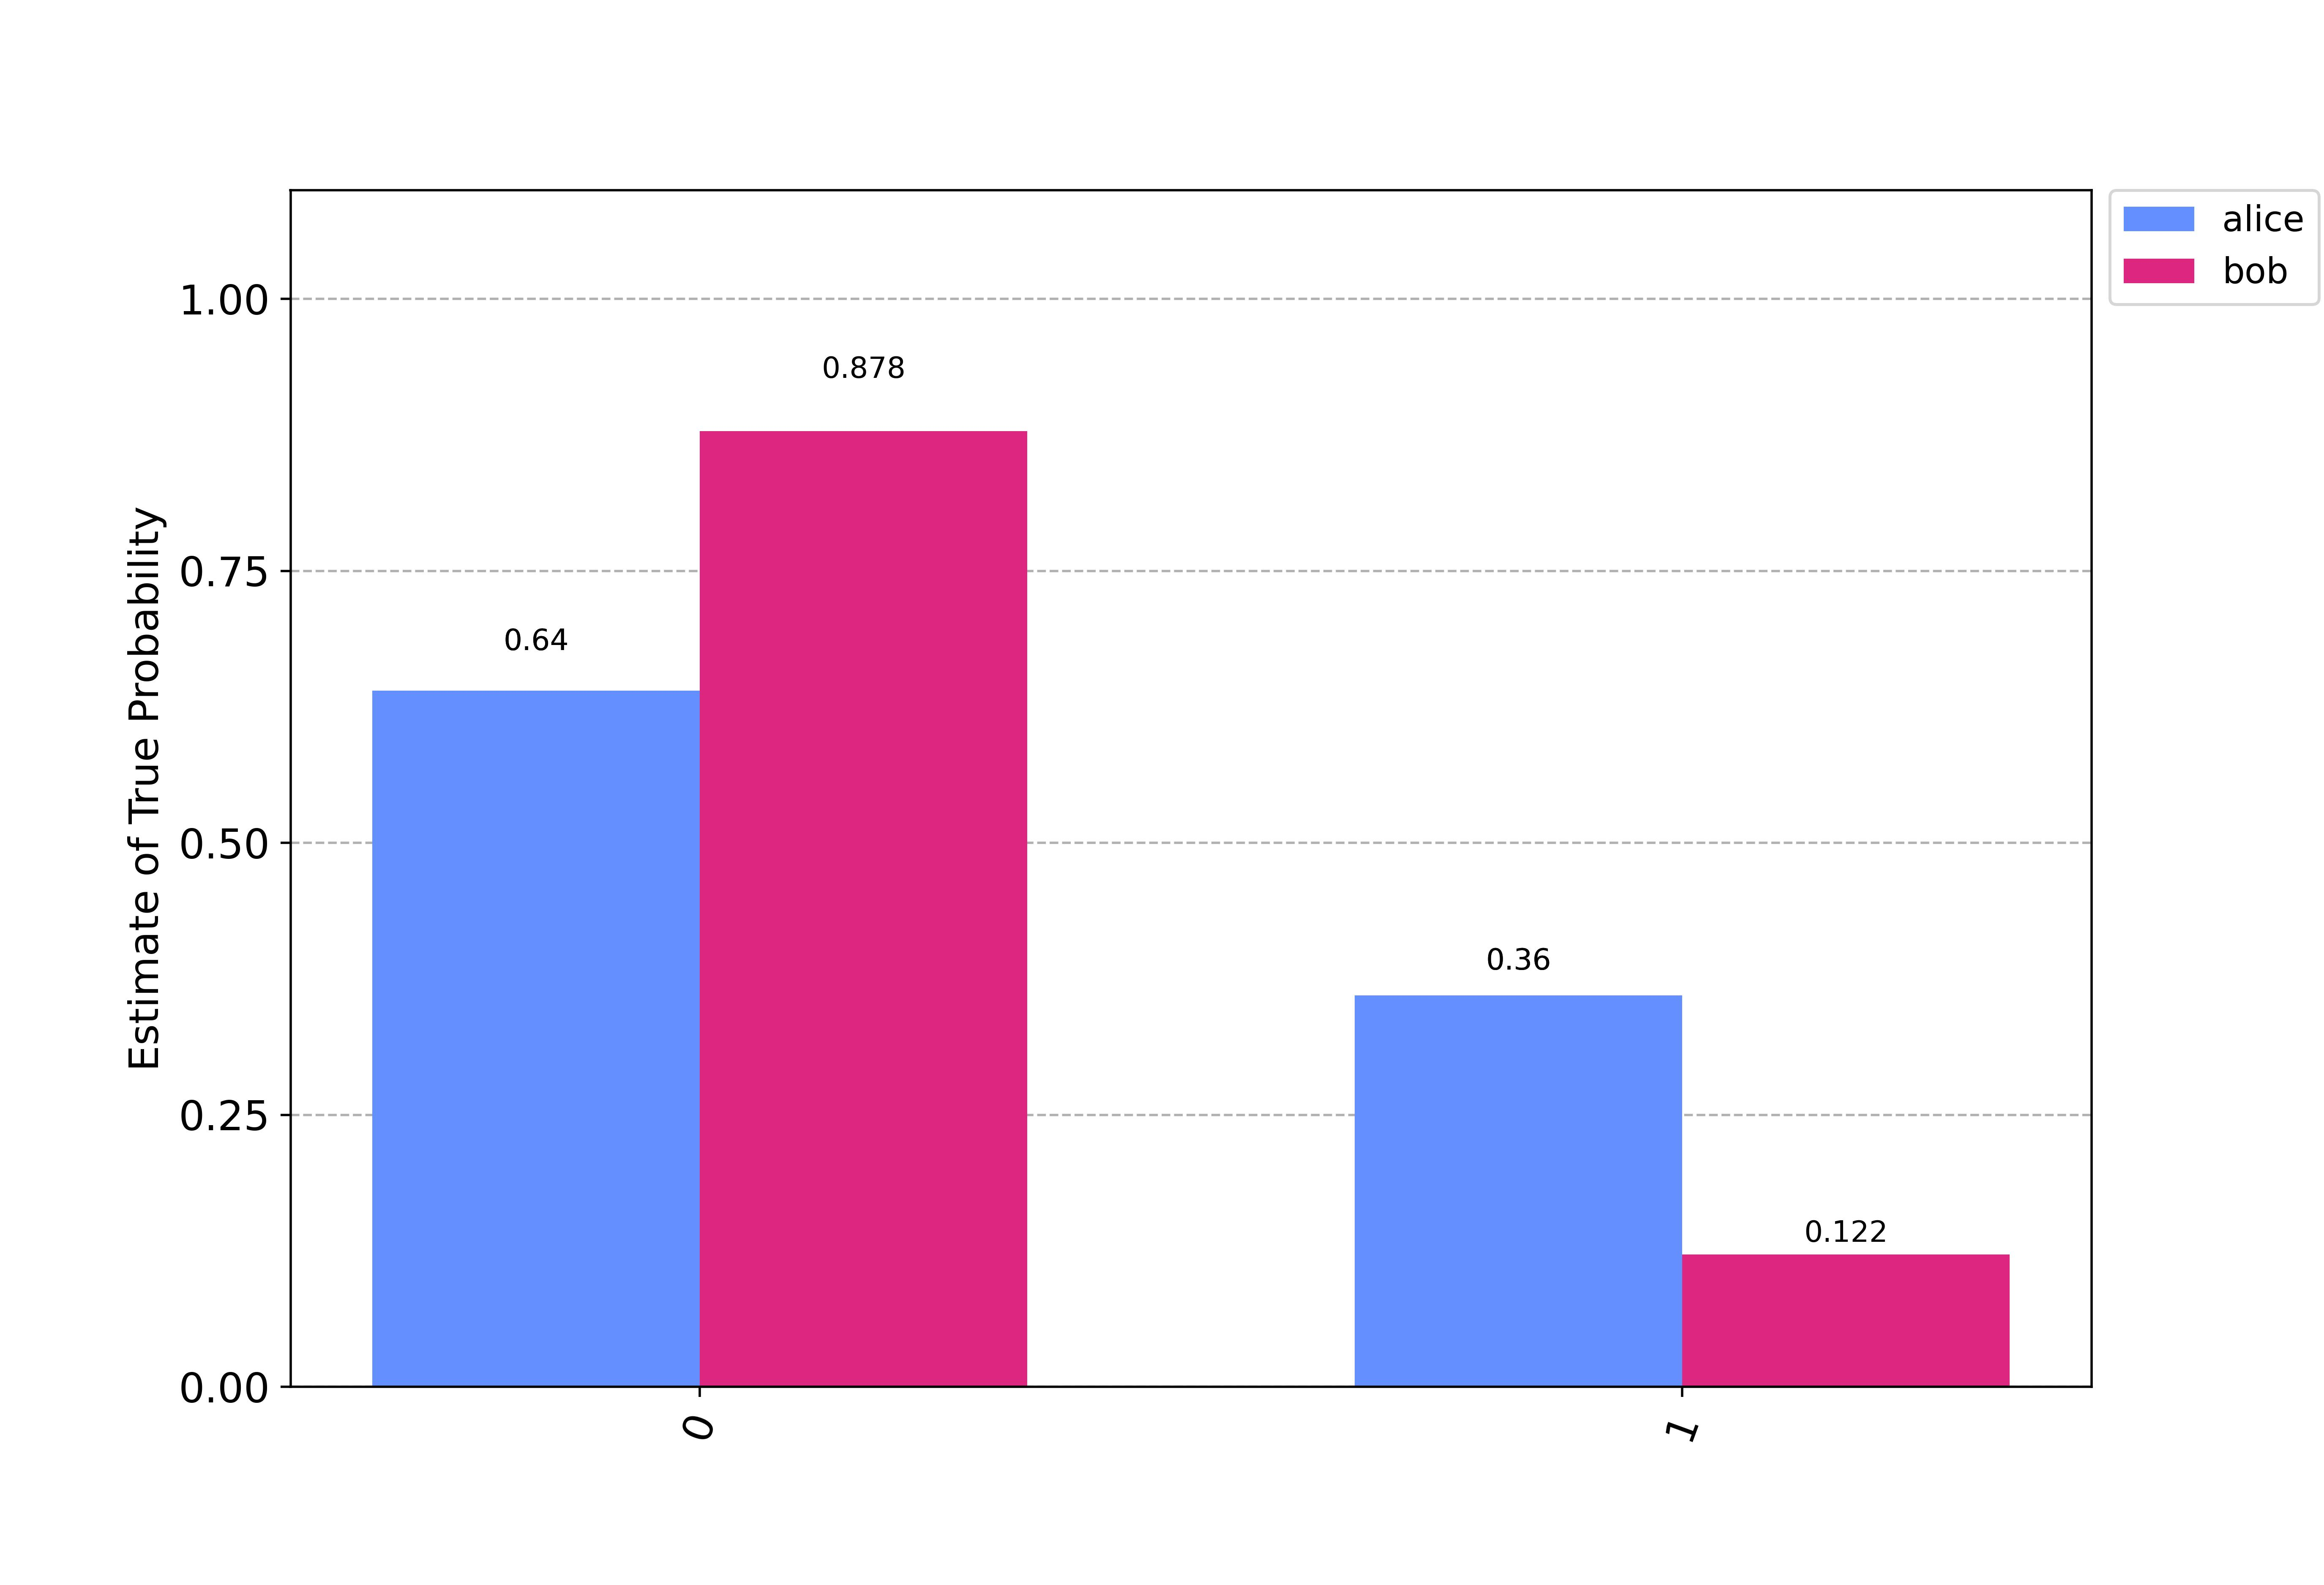
\includegraphics[width=\linewidth]{figures/dps_verification_post_bell_pair.jpg}
    \caption{Post Bell-pair production purification strategy}
    \label{fig:deutsch_purification_strategy_verification_results_post_bell_pair}
  \end{subfigure}
  \begin{subfigure}[b]{0.45\textwidth}
    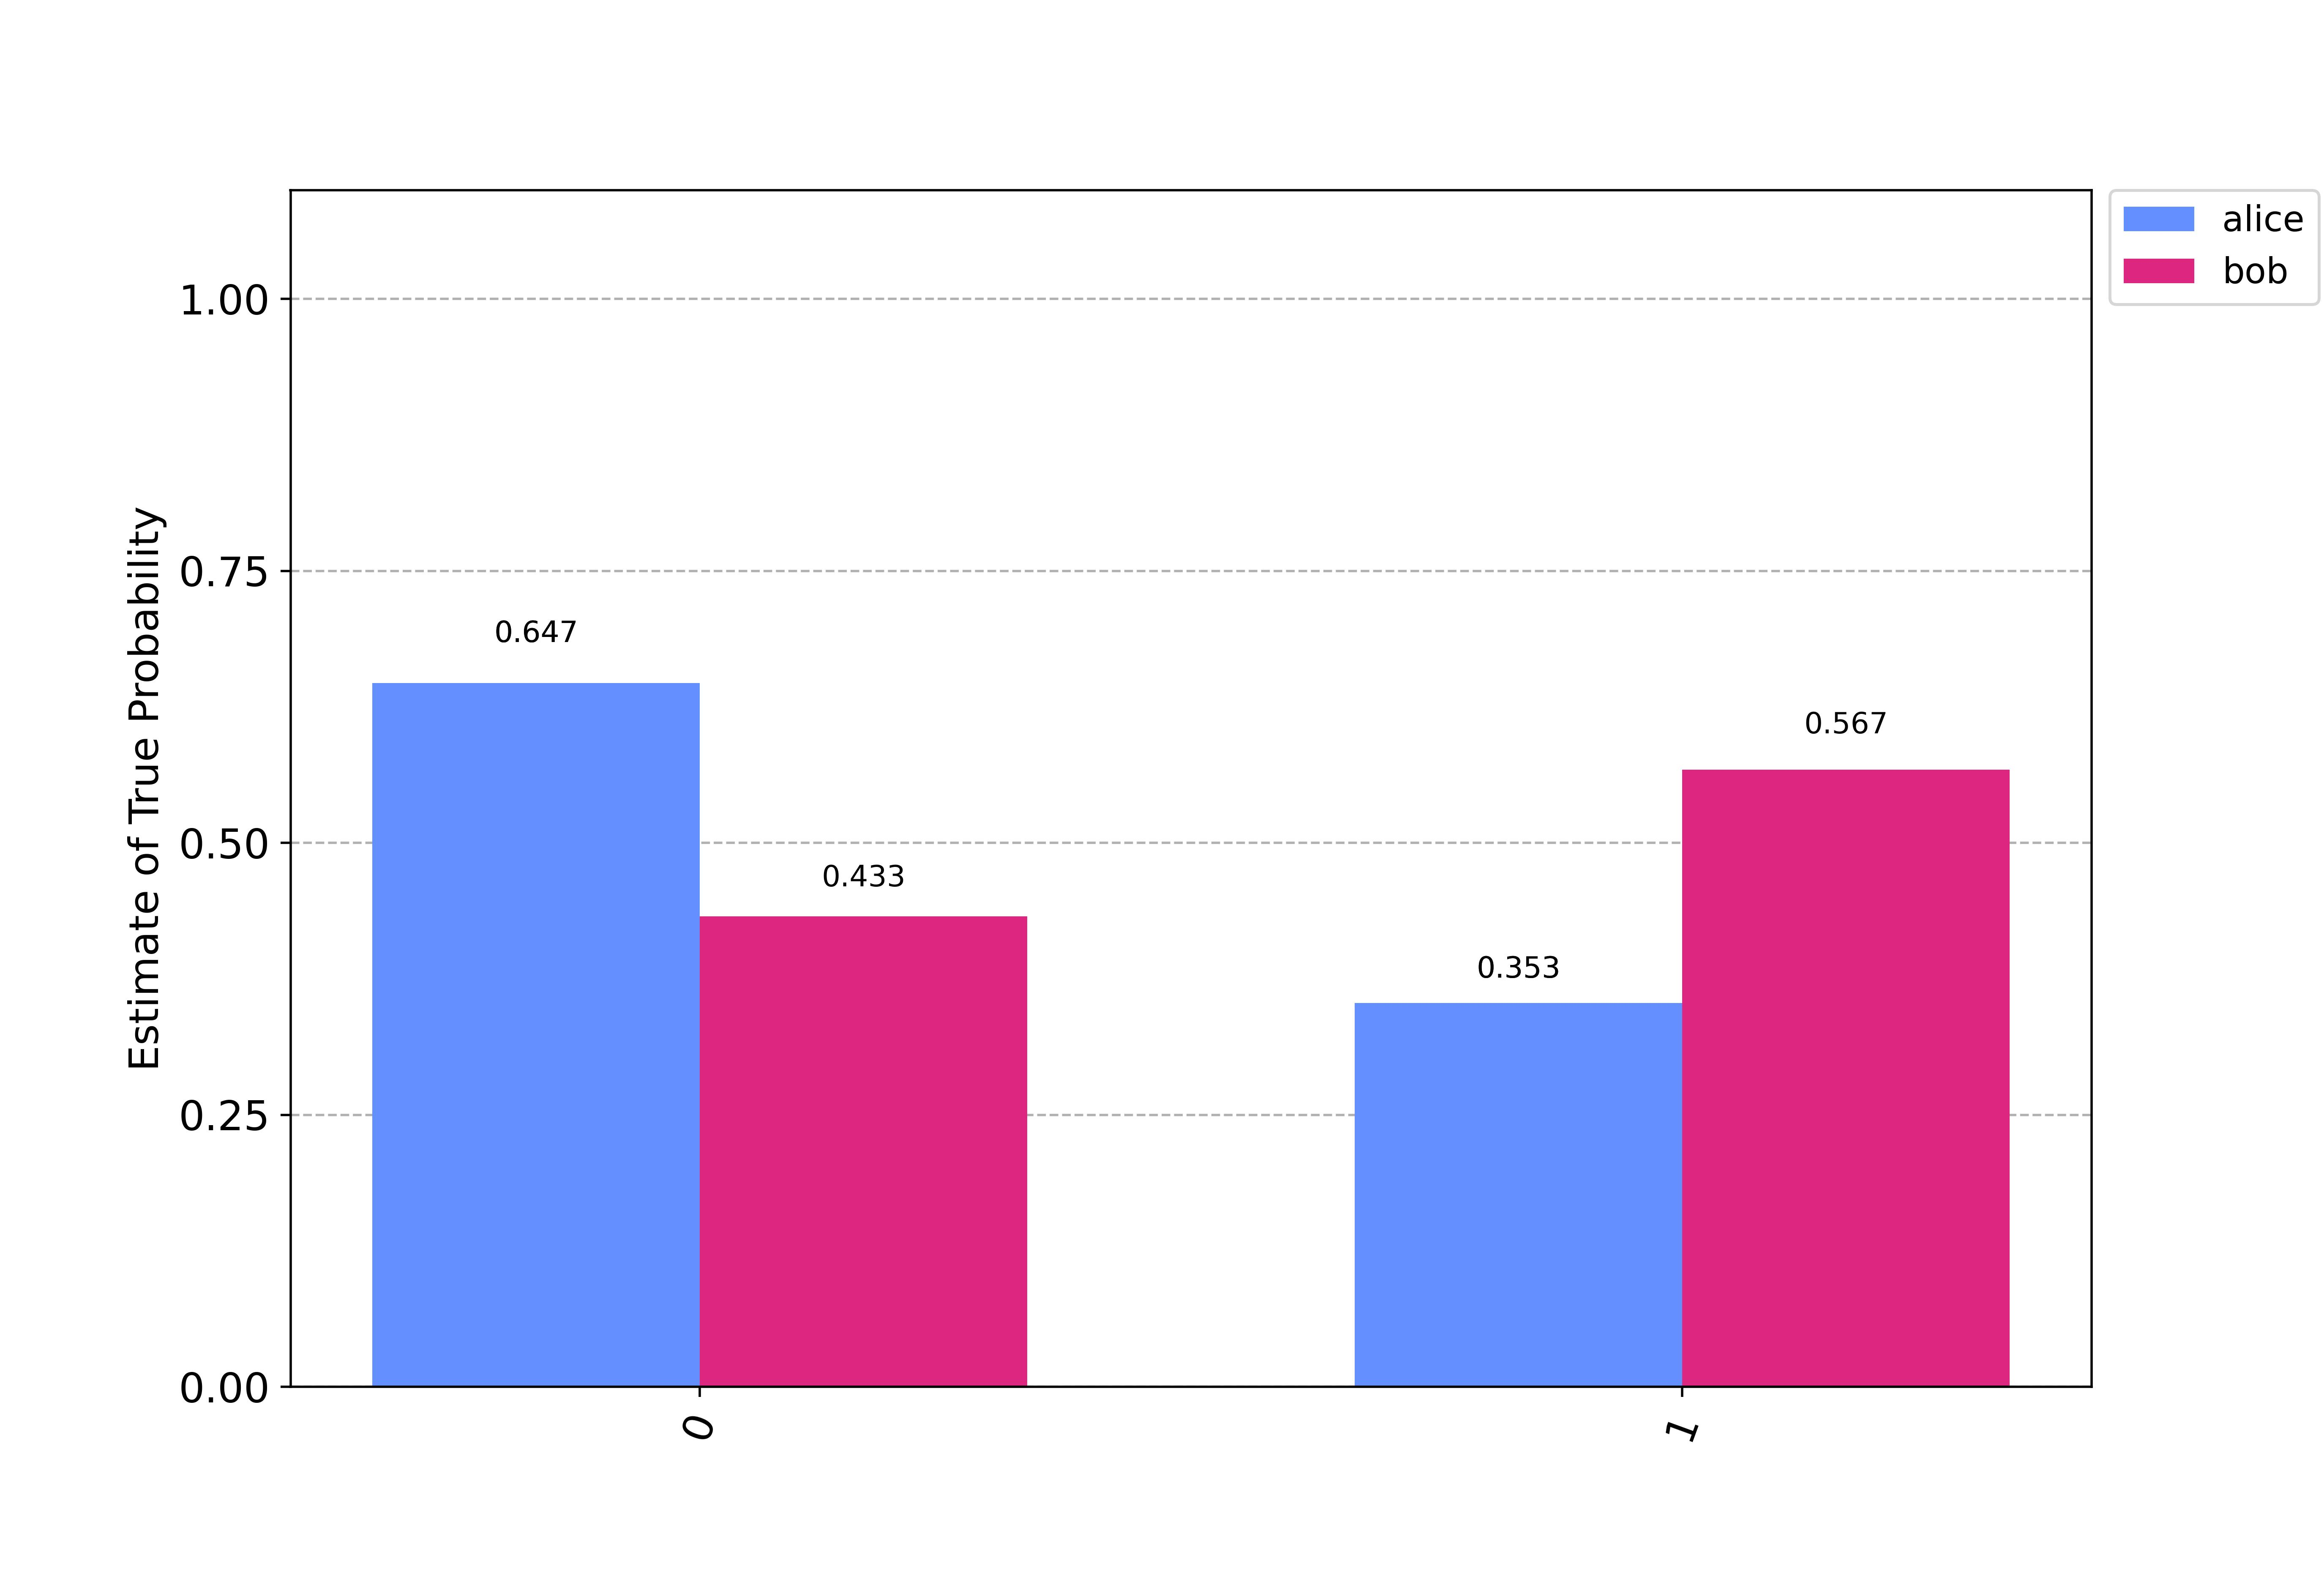
\includegraphics[width=\linewidth]{figures/dps_verification_post_swap.jpg}
    \caption{Post swap purification strategy}
    \label{fig:deutsch_purification_strategy_verification_results_post_swap}
  \end{subfigure}
  \\
  \begin{subfigure}[b]{0.45\textwidth}
    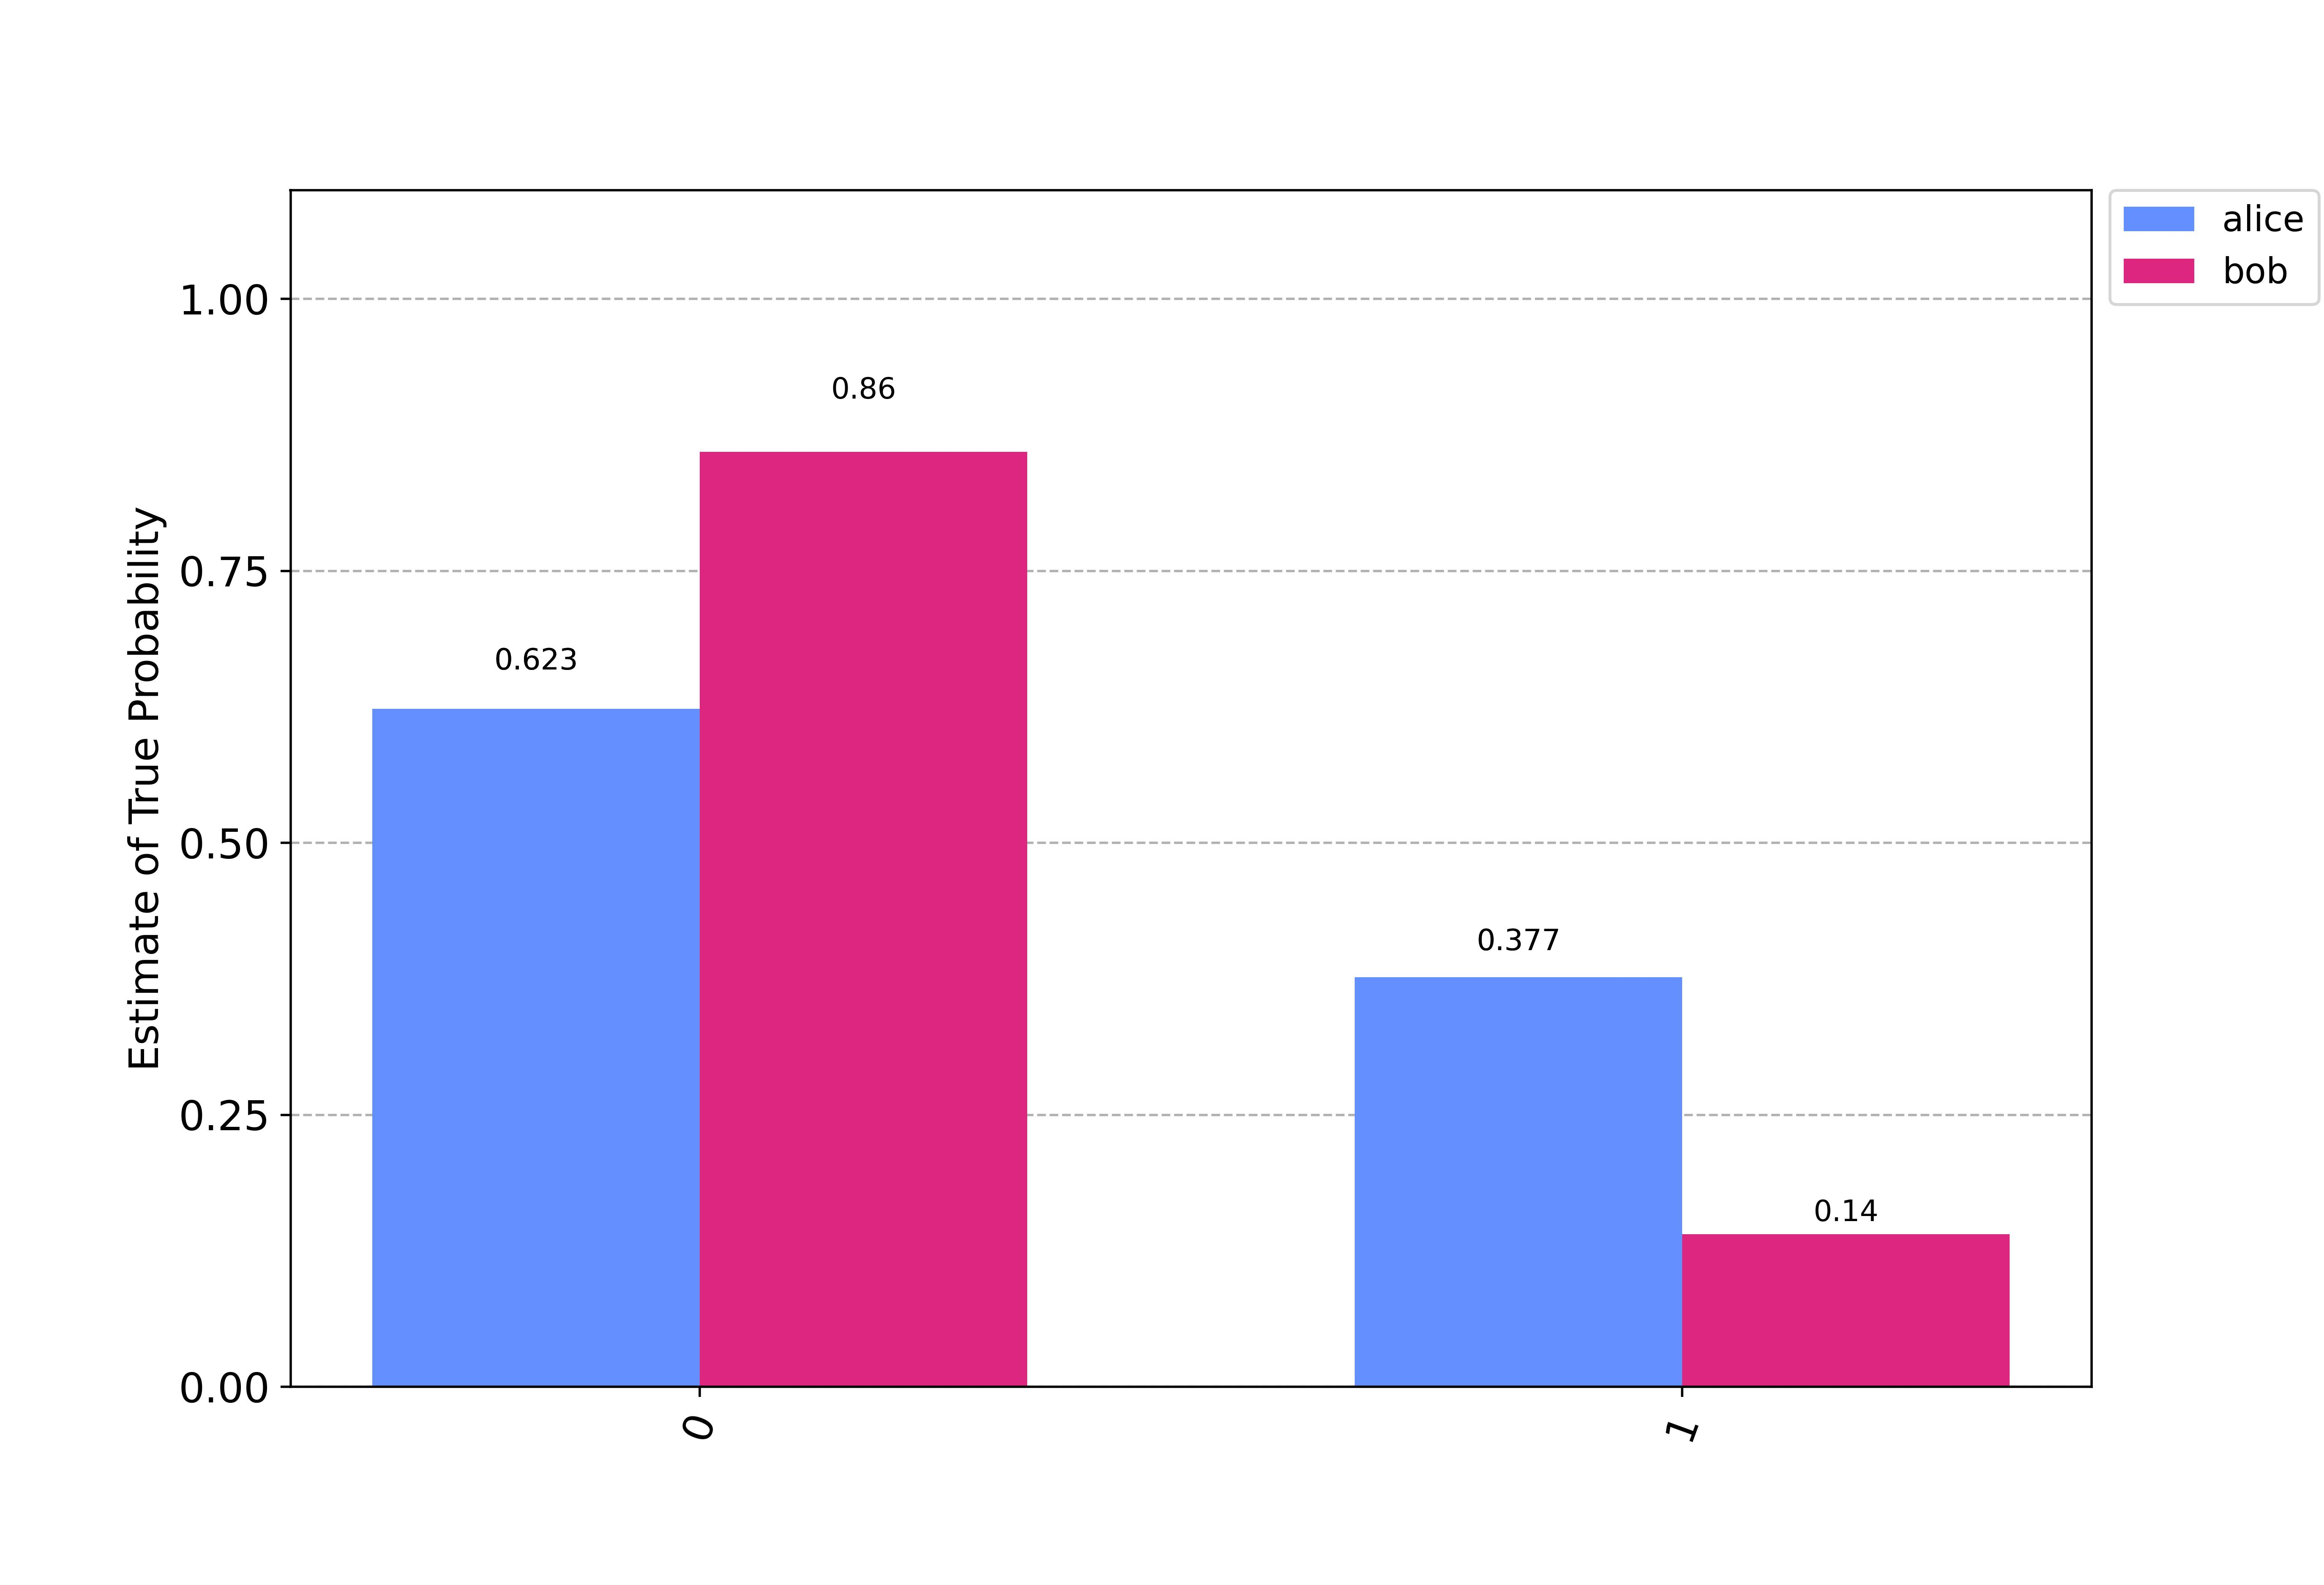
\includegraphics[width=\linewidth]{figures/dps_verification_pre_and_post_swap.jpg}
    \caption{Pre-and-post swap purification strategy}
    \label{fig:deutsch_purification_strategy_verification_results_pre_post_swap}
  \end{subfigure}
  \begin{subfigure}[b]{0.45\textwidth}
    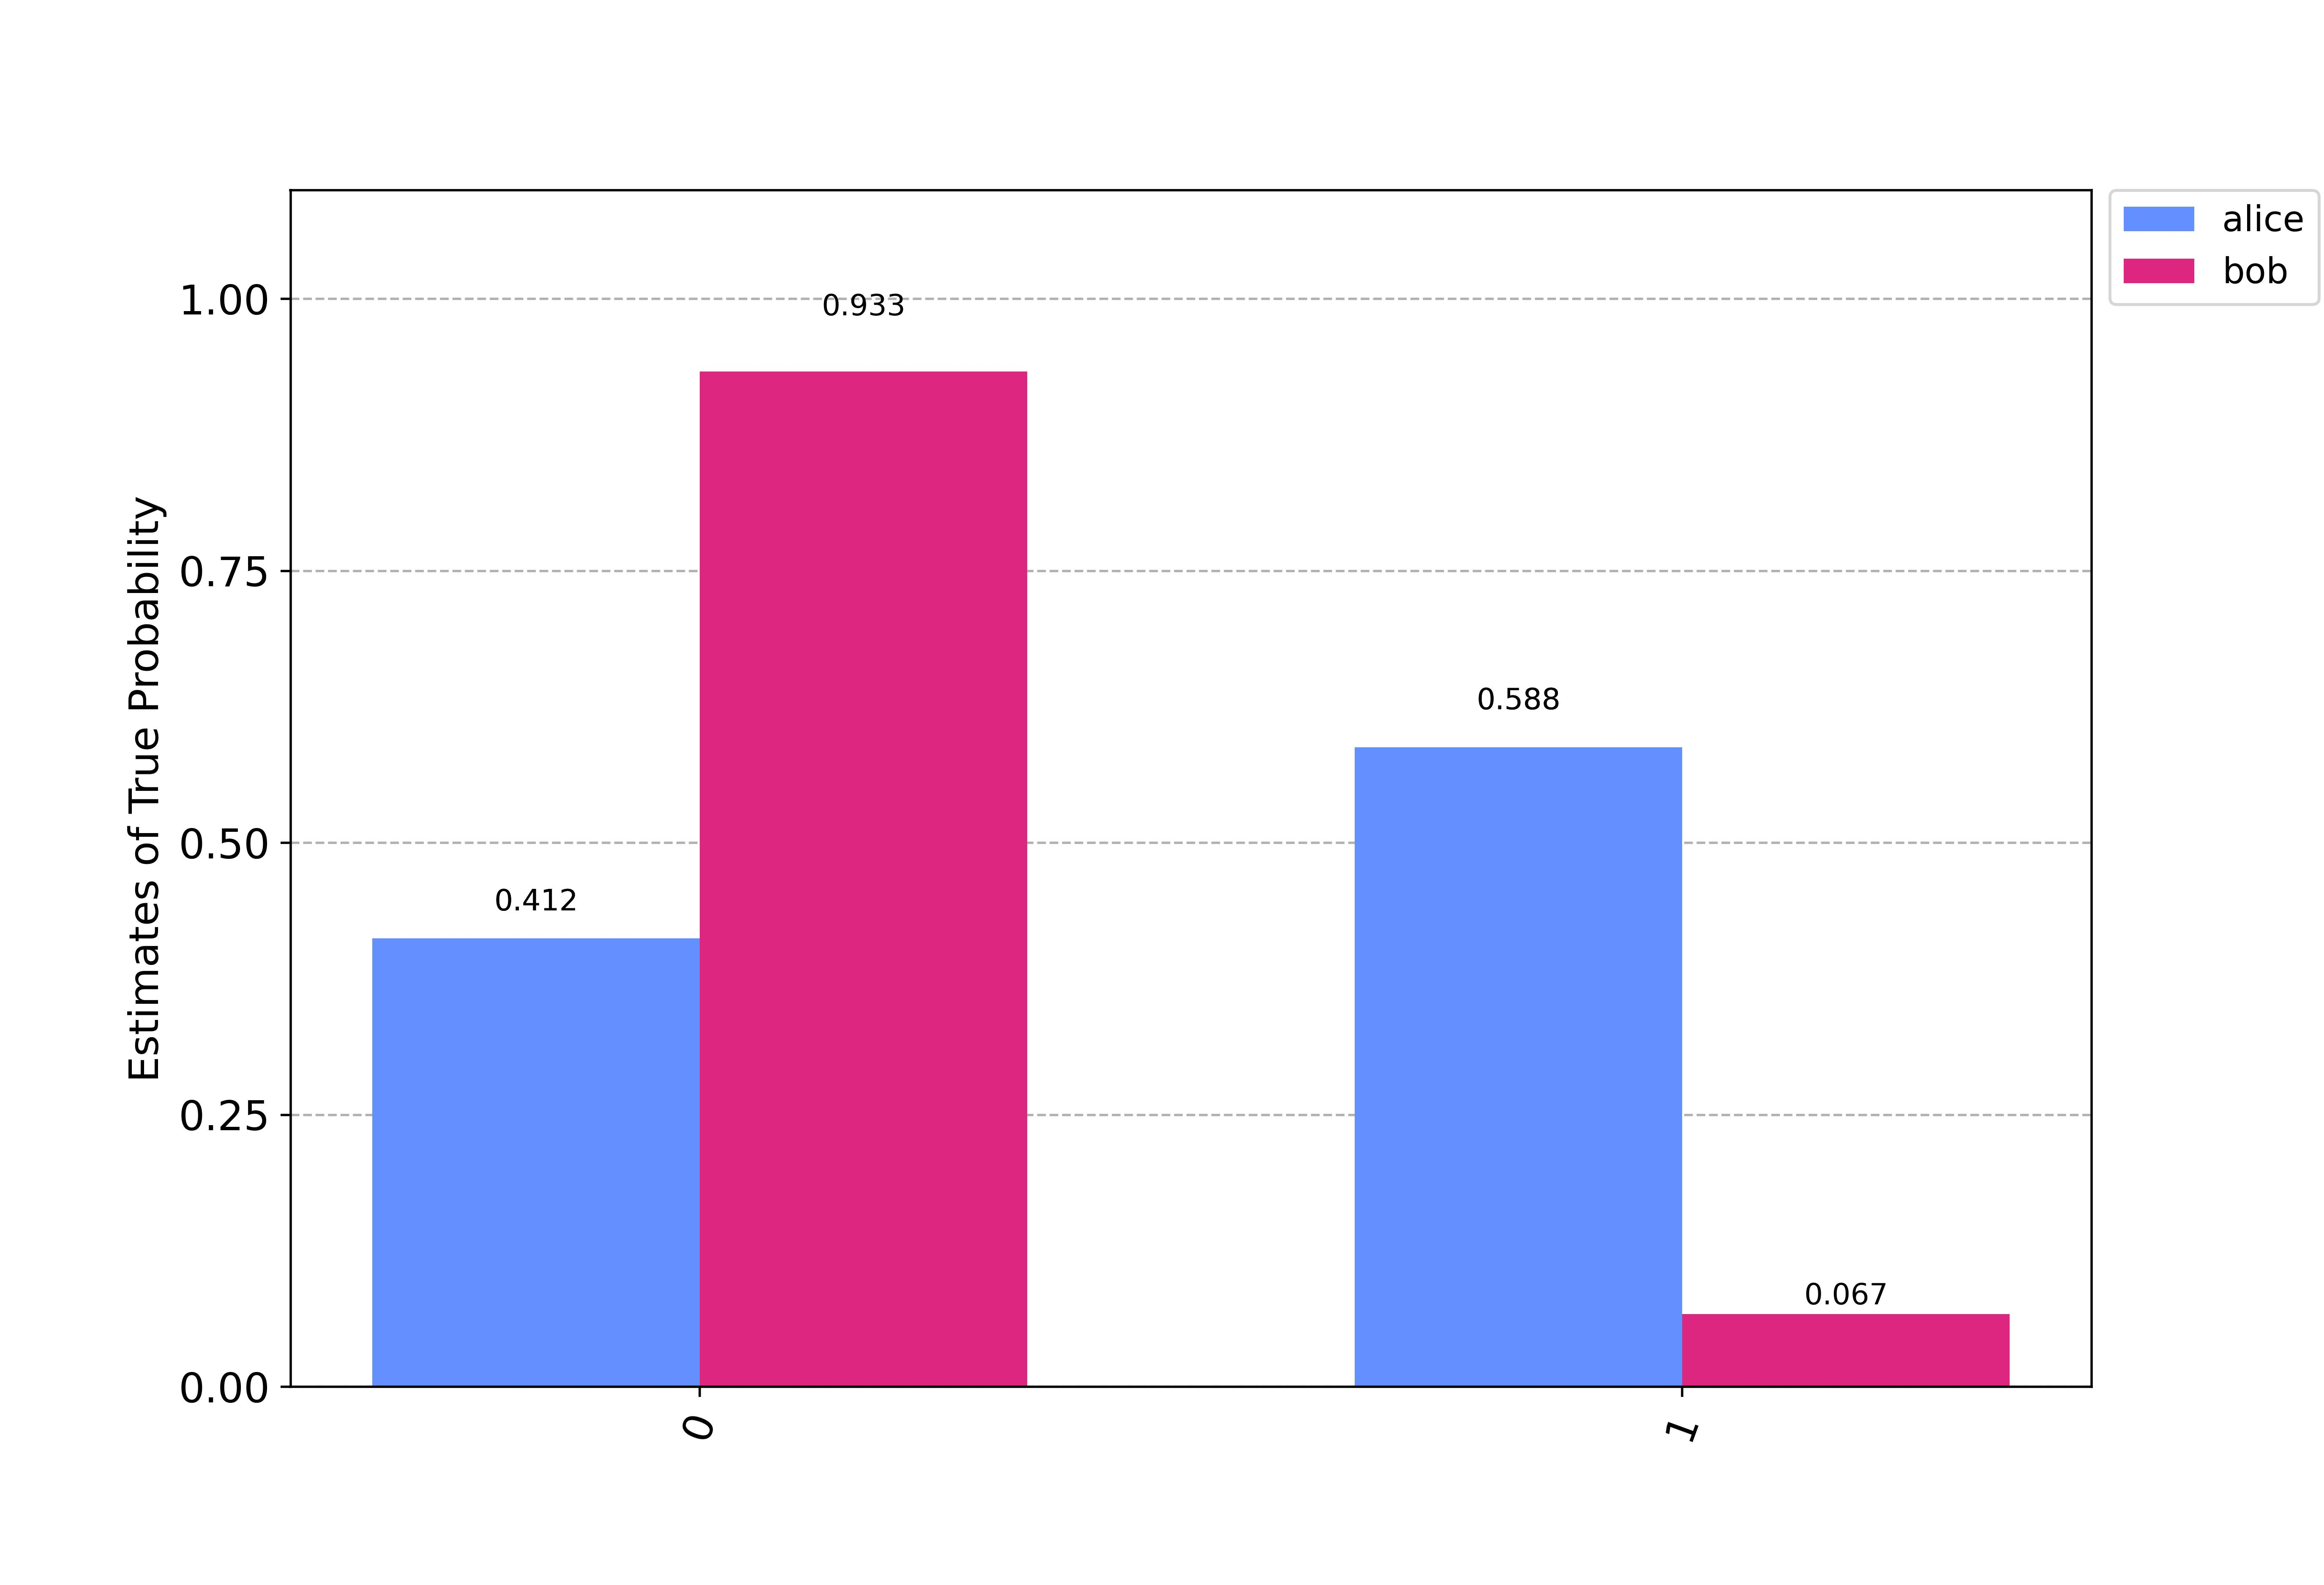
\includegraphics[width=\linewidth]{figures/dps_verification_repeated_post_swap.jpg}
    \caption{Repeated post swap purification strategy}
    \label{fig:deutsch_purification_strategy_verification_results_repeated_post_swap}
  \end{subfigure}
  \caption[Verification of teleportation in quantum Repeater protocol]{Results verifying the success of the teleportation of entanglement in the quantum repeater protocol between Alice and Bob under different purification strategies as indicated in each graph.}
  \label{fig:deutsch_purification_strategy_verification_results}
\end{figure}

Figure \ref{fig:deutsch_purification_strategy}, shows the results of the impact purification had on the fidelity at different stages in the quantum repeater protocol. The considered stages are: distribution stage denoted \textit{dist}, first swapping stage denoted \textit{aswap1}, second swapping stage denoted \textit{aswap2} and eventually the end of the node. At each stage, we obtained the fidelity of the quantum circuit. This was done by creating a duplicate of the quantum circuit covered up to each specific stage then executing that circuit and performing measurements on it. This was repeated for the 20 runs of the simulation. There then were 20 independent measurement results each with 4 measurement results from the 4 stages considered. The results were then averaged out before performing the Hellinger fidelity operation to obtain the fidelity between each two stages in sequence.

From observation, entanglement distribution has little effect on the fidelity. The fidelity of the Bell-pairs takes a hit during entanglement swapping and readout at the end of the node.
\begin{figure}[ht]
    \centering
    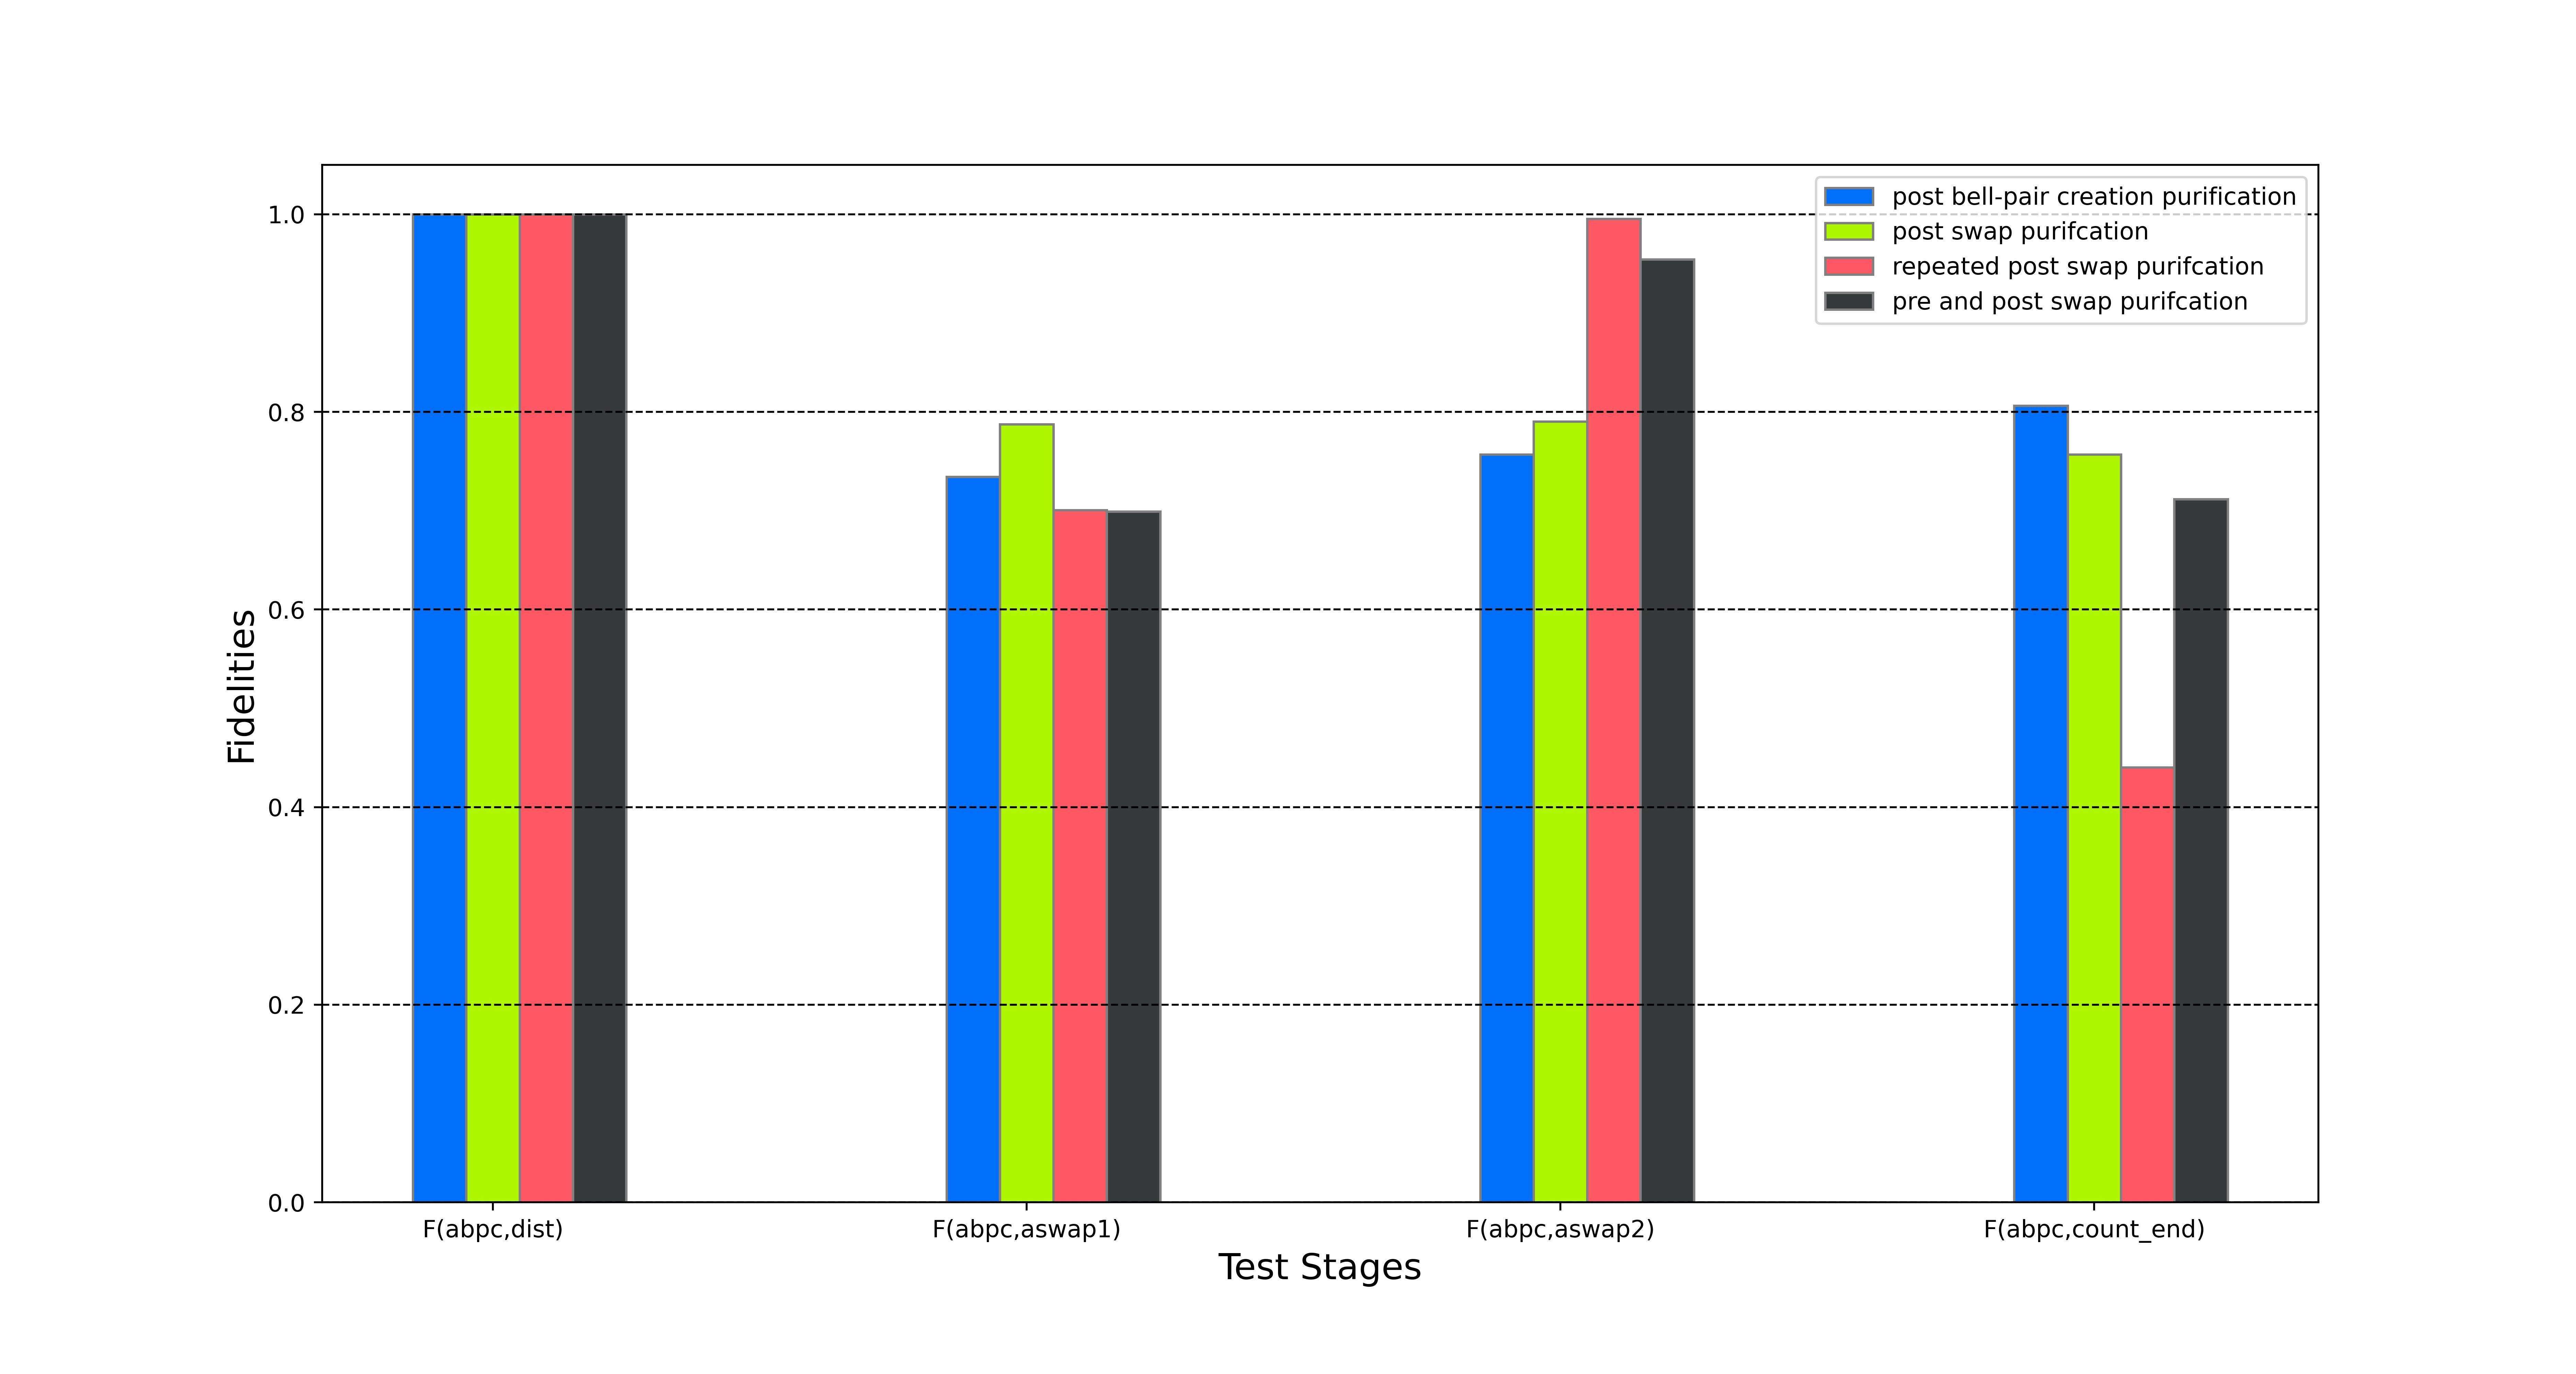
\includegraphics[width=\textwidth]{figures/deutsch_purification_strategy.jpg}
    \caption[Purification strategy]{Effect of purification on fidelity across different purification strategies. The results were obtained from a circuit implementing one intermediate quantum repeater and hence two entanglement swapping procedures, labelled as \textit{aswap1} and \textit{aswap2}.}
    \label{fig:deutsch_purification_strategy}
\end{figure}

The post swap purification strategy looks favourable based on how it is able to maintain a relatively consistent fidelity throughout the quantum repeater protocol. The repeated post swap purification strategy suffers a very low fidelity at the readout state. Such low fidelities especially below $50\%$ are unfavourable for maintaining the quantum communication link. The fidelities posted by the rest of the purification strategies at different stages indicate that they can be applied in a quantum repeater and be able to maintain a communication link.

Combining all the data collected, we gain insight into the optimum purification strategy. Both the post Bell-pair production purification strategy and the pre and post swap purification strategy emerge as the most favourable of the strategies considered. Both had a high estimate of probability in the measurement results of Alice's and Bob's qubits (see Figure \ref{fig:deutsch_measurement_strategy_results}). Both maintained a high estimate of probability for the verification of quantum repeater protocol results as seen in Figure \ref{fig:deutsch_purification_strategy_verification_results}. Their measurement on Bob's qubit being in the $|0\rangle$ state were the highest. Lastly, the fidelities as seen in Figure \ref{fig:deutsch_purification_strategy} are well maintained at higher percentages.

\subsection{Purification Optimization Scheme}
The purification circuits underwent two levels of optimization - a light optimization scheme and a heavy optimization scheme. The IBM Qiskit transpiler is responsible for the optimization levels used. The purification optimization scheme was carried out for all purification strategies tested out earlier using the two major purification protocols - Bennett's and Deutsch's protocols.

For each of the 4 purification strategies, the circuit would first implement Deutsch's purification protocol starting with light optimization then the execution would be repeated using heavy optimization, followed by Bennett's purification protocol with both the light and heavy optimization schemes.
\begin{figure}[ht]
  \centering
  \begin{subfigure}[b]{0.45\textwidth}
    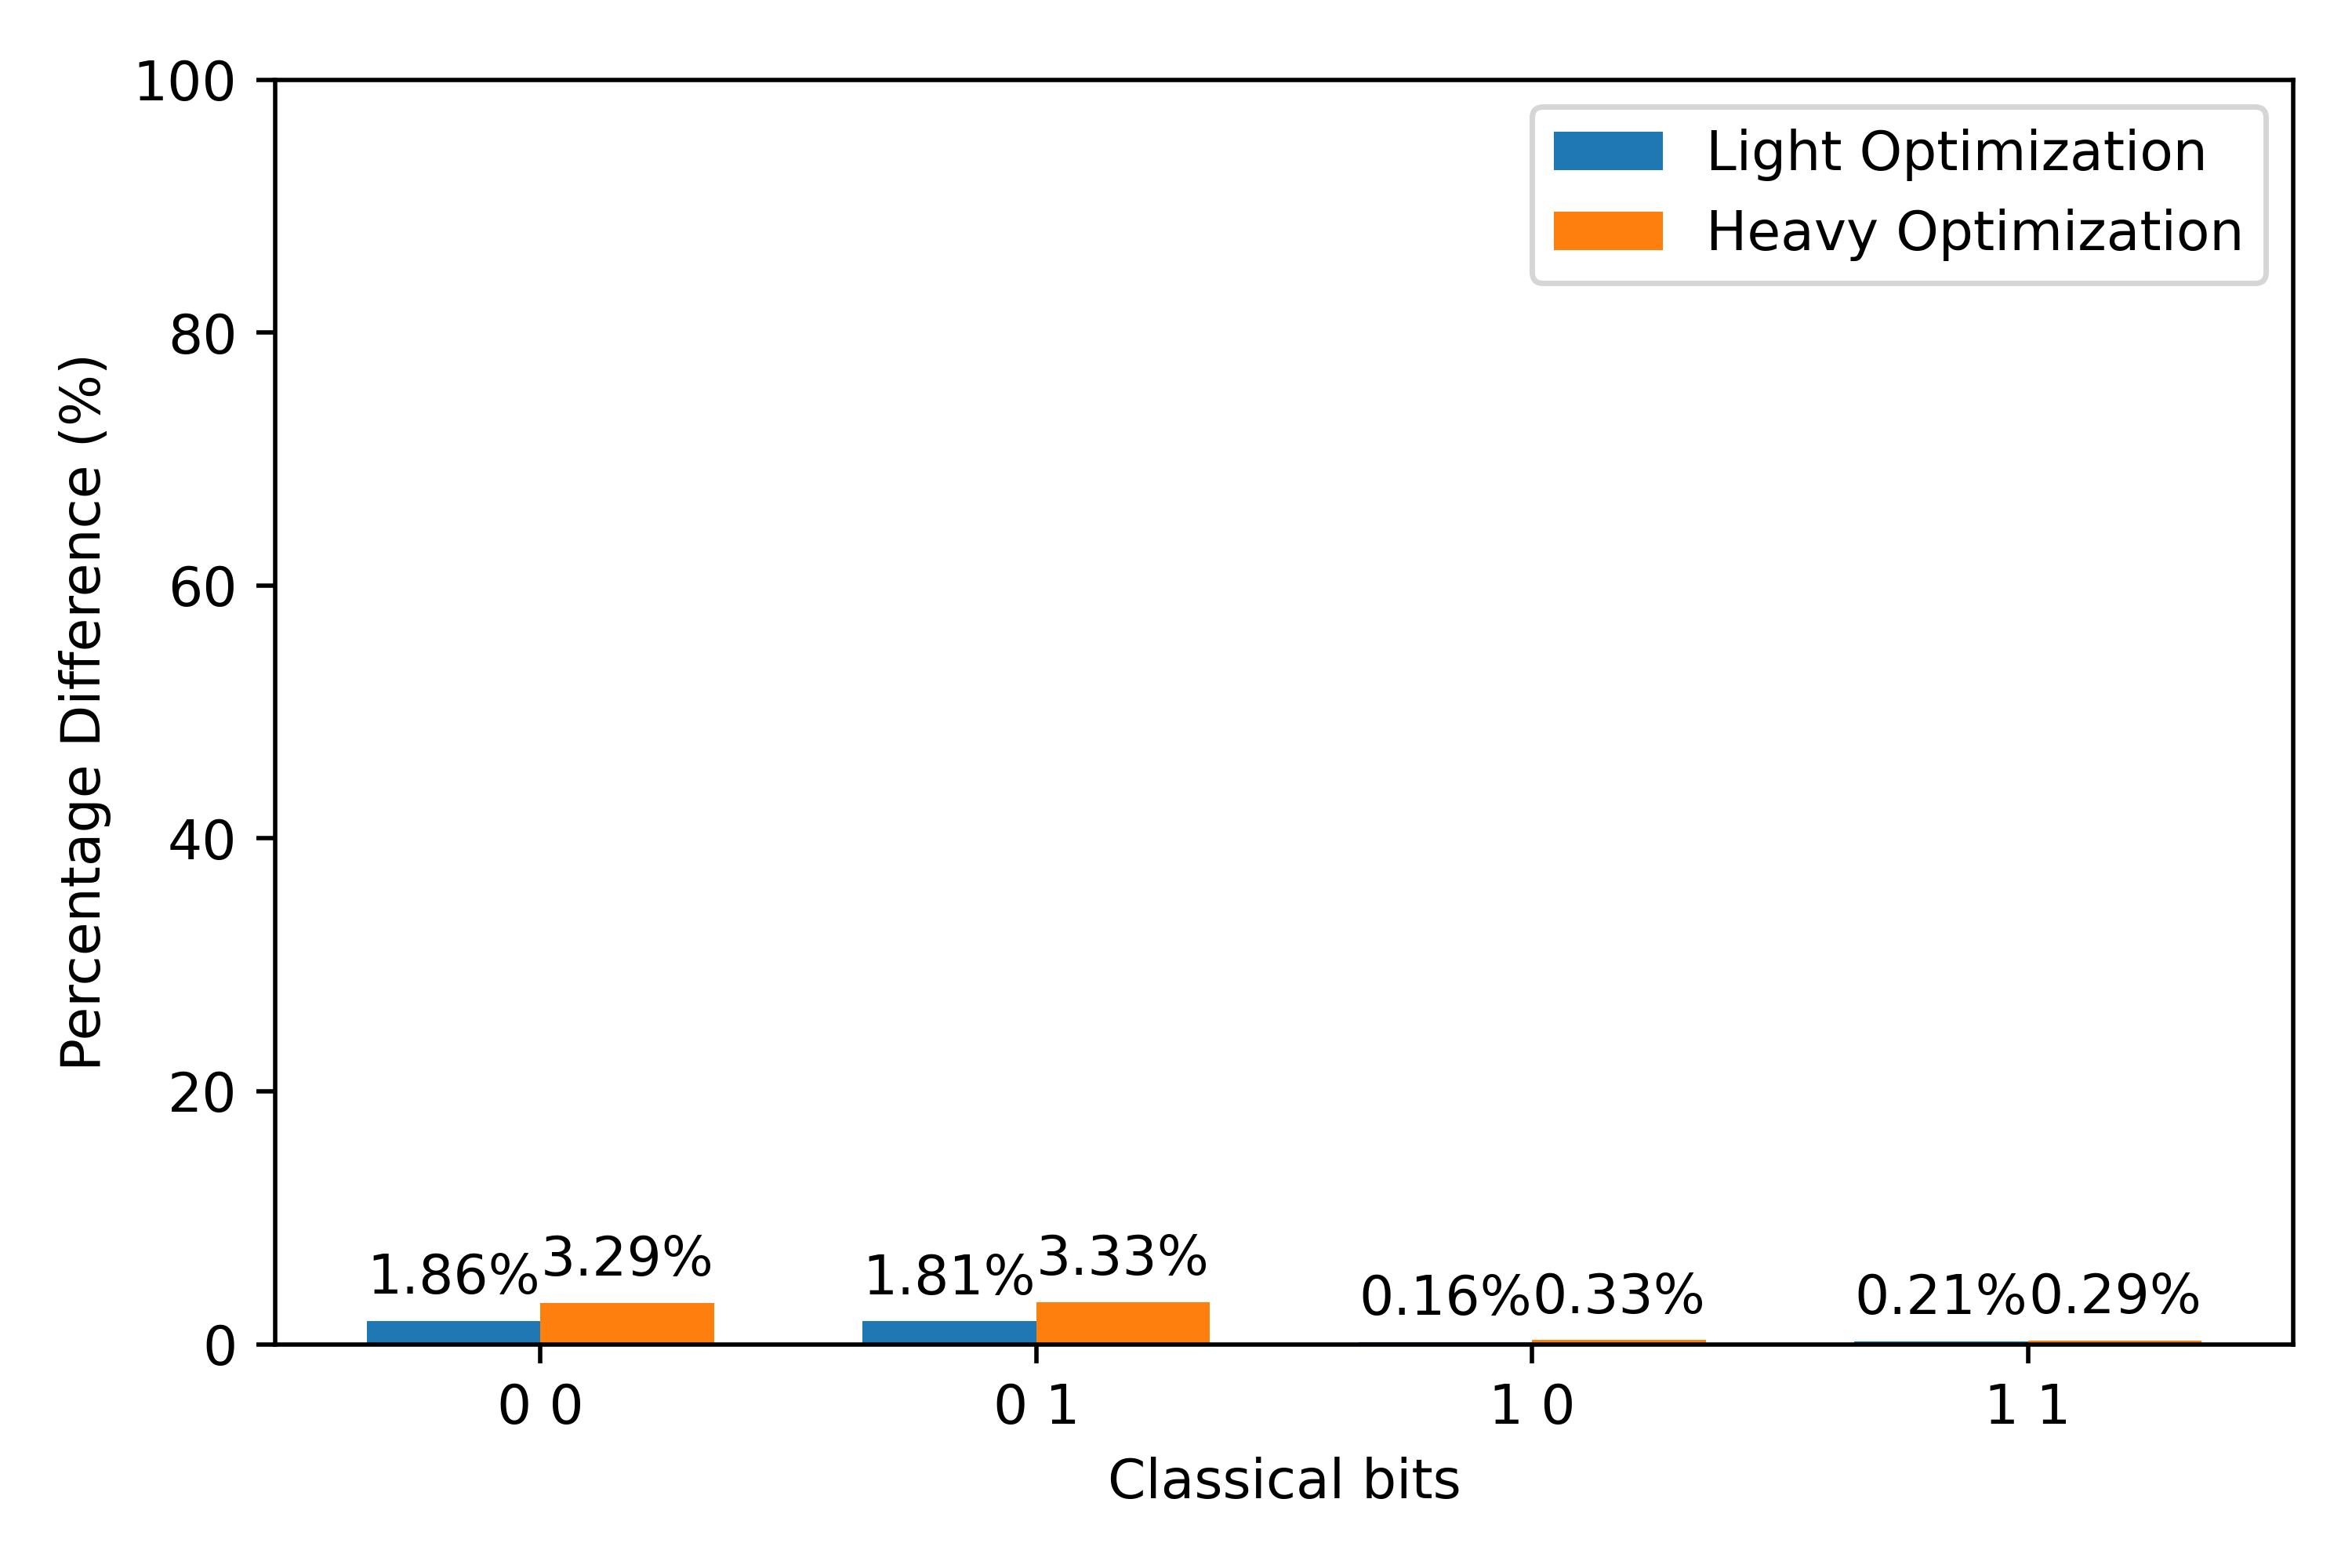
\includegraphics[width=\linewidth]{figures/po_post_bell_pair.jpg}
    \caption{Post Bell-Pair}
    \label{fig:po_all_post_bell_pair}
  \end{subfigure}
  \begin{subfigure}[b]{0.45\textwidth}
    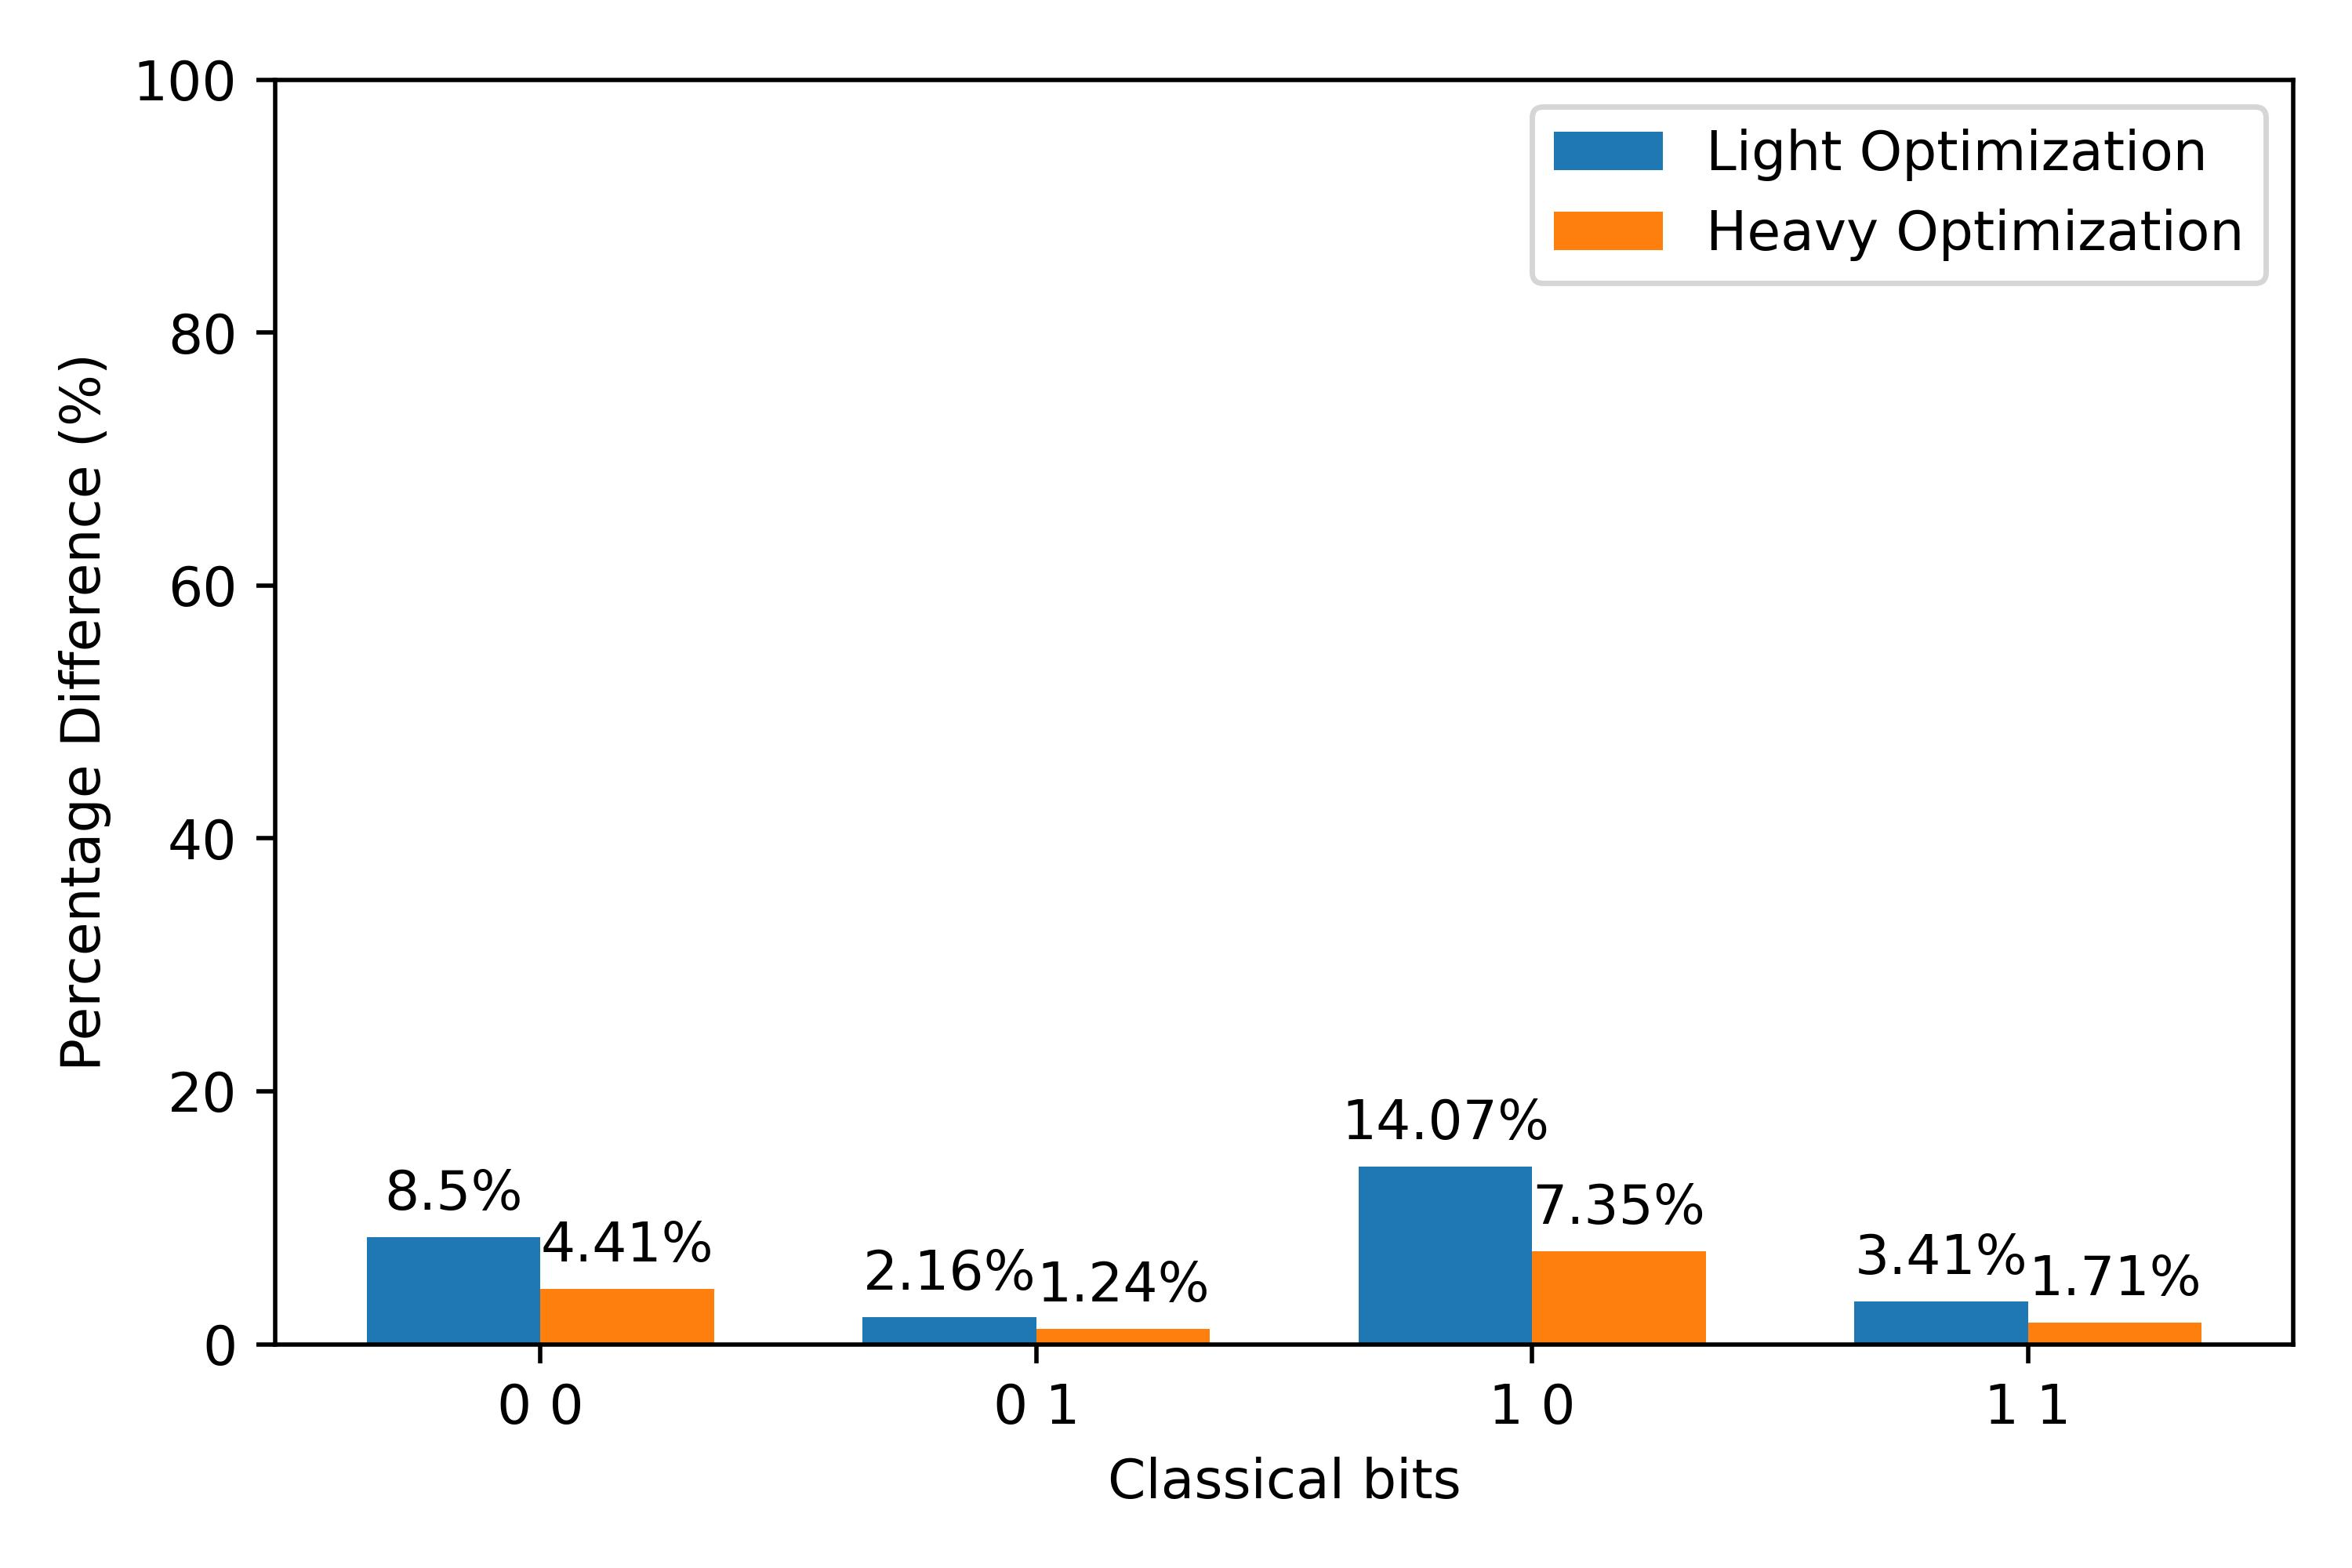
\includegraphics[width=\linewidth]{figures/po_post_swap.jpg}
    \caption{Post swap}
    \label{fig:po_all_post_swap}
  \end{subfigure}
  \\
  \begin{subfigure}[b]{0.45\textwidth}
    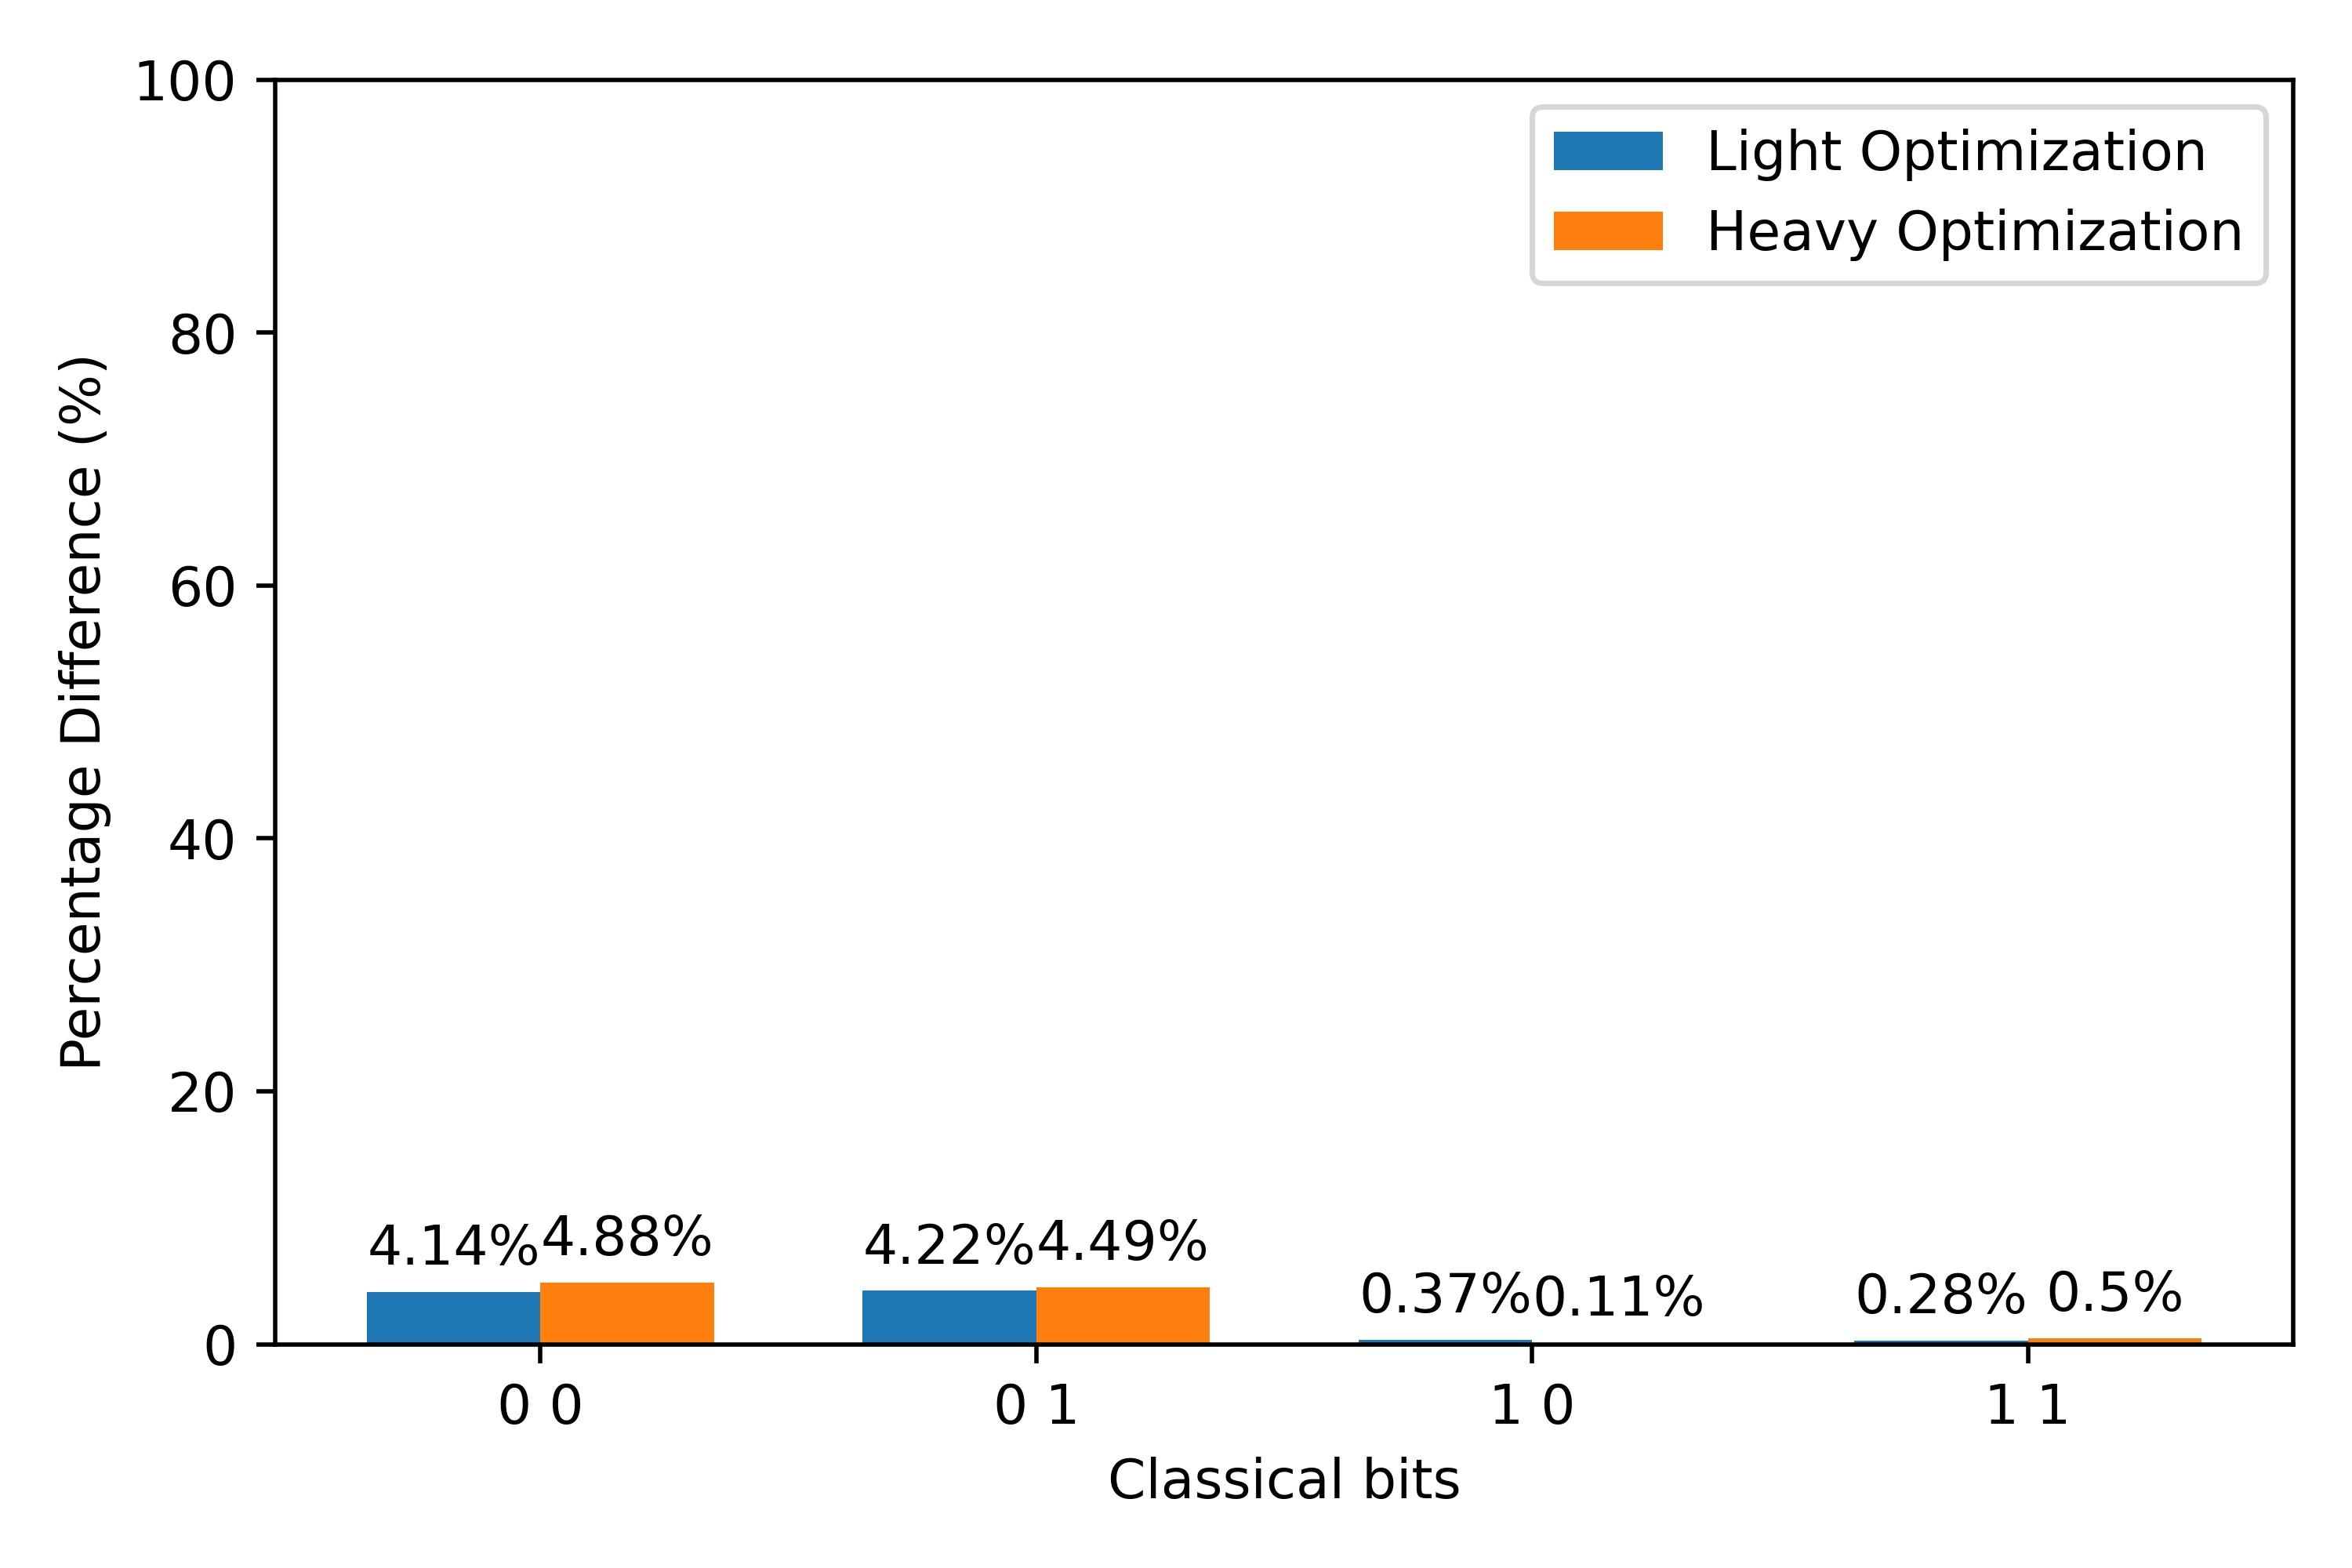
\includegraphics[width=\linewidth]{figures/po_pre_and_post_swap.jpg}
    \caption{Pre-and-post swap}
    \label{fig:po_all_pre_post_swap}
  \end{subfigure}
  \begin{subfigure}[b]{0.45\textwidth}
    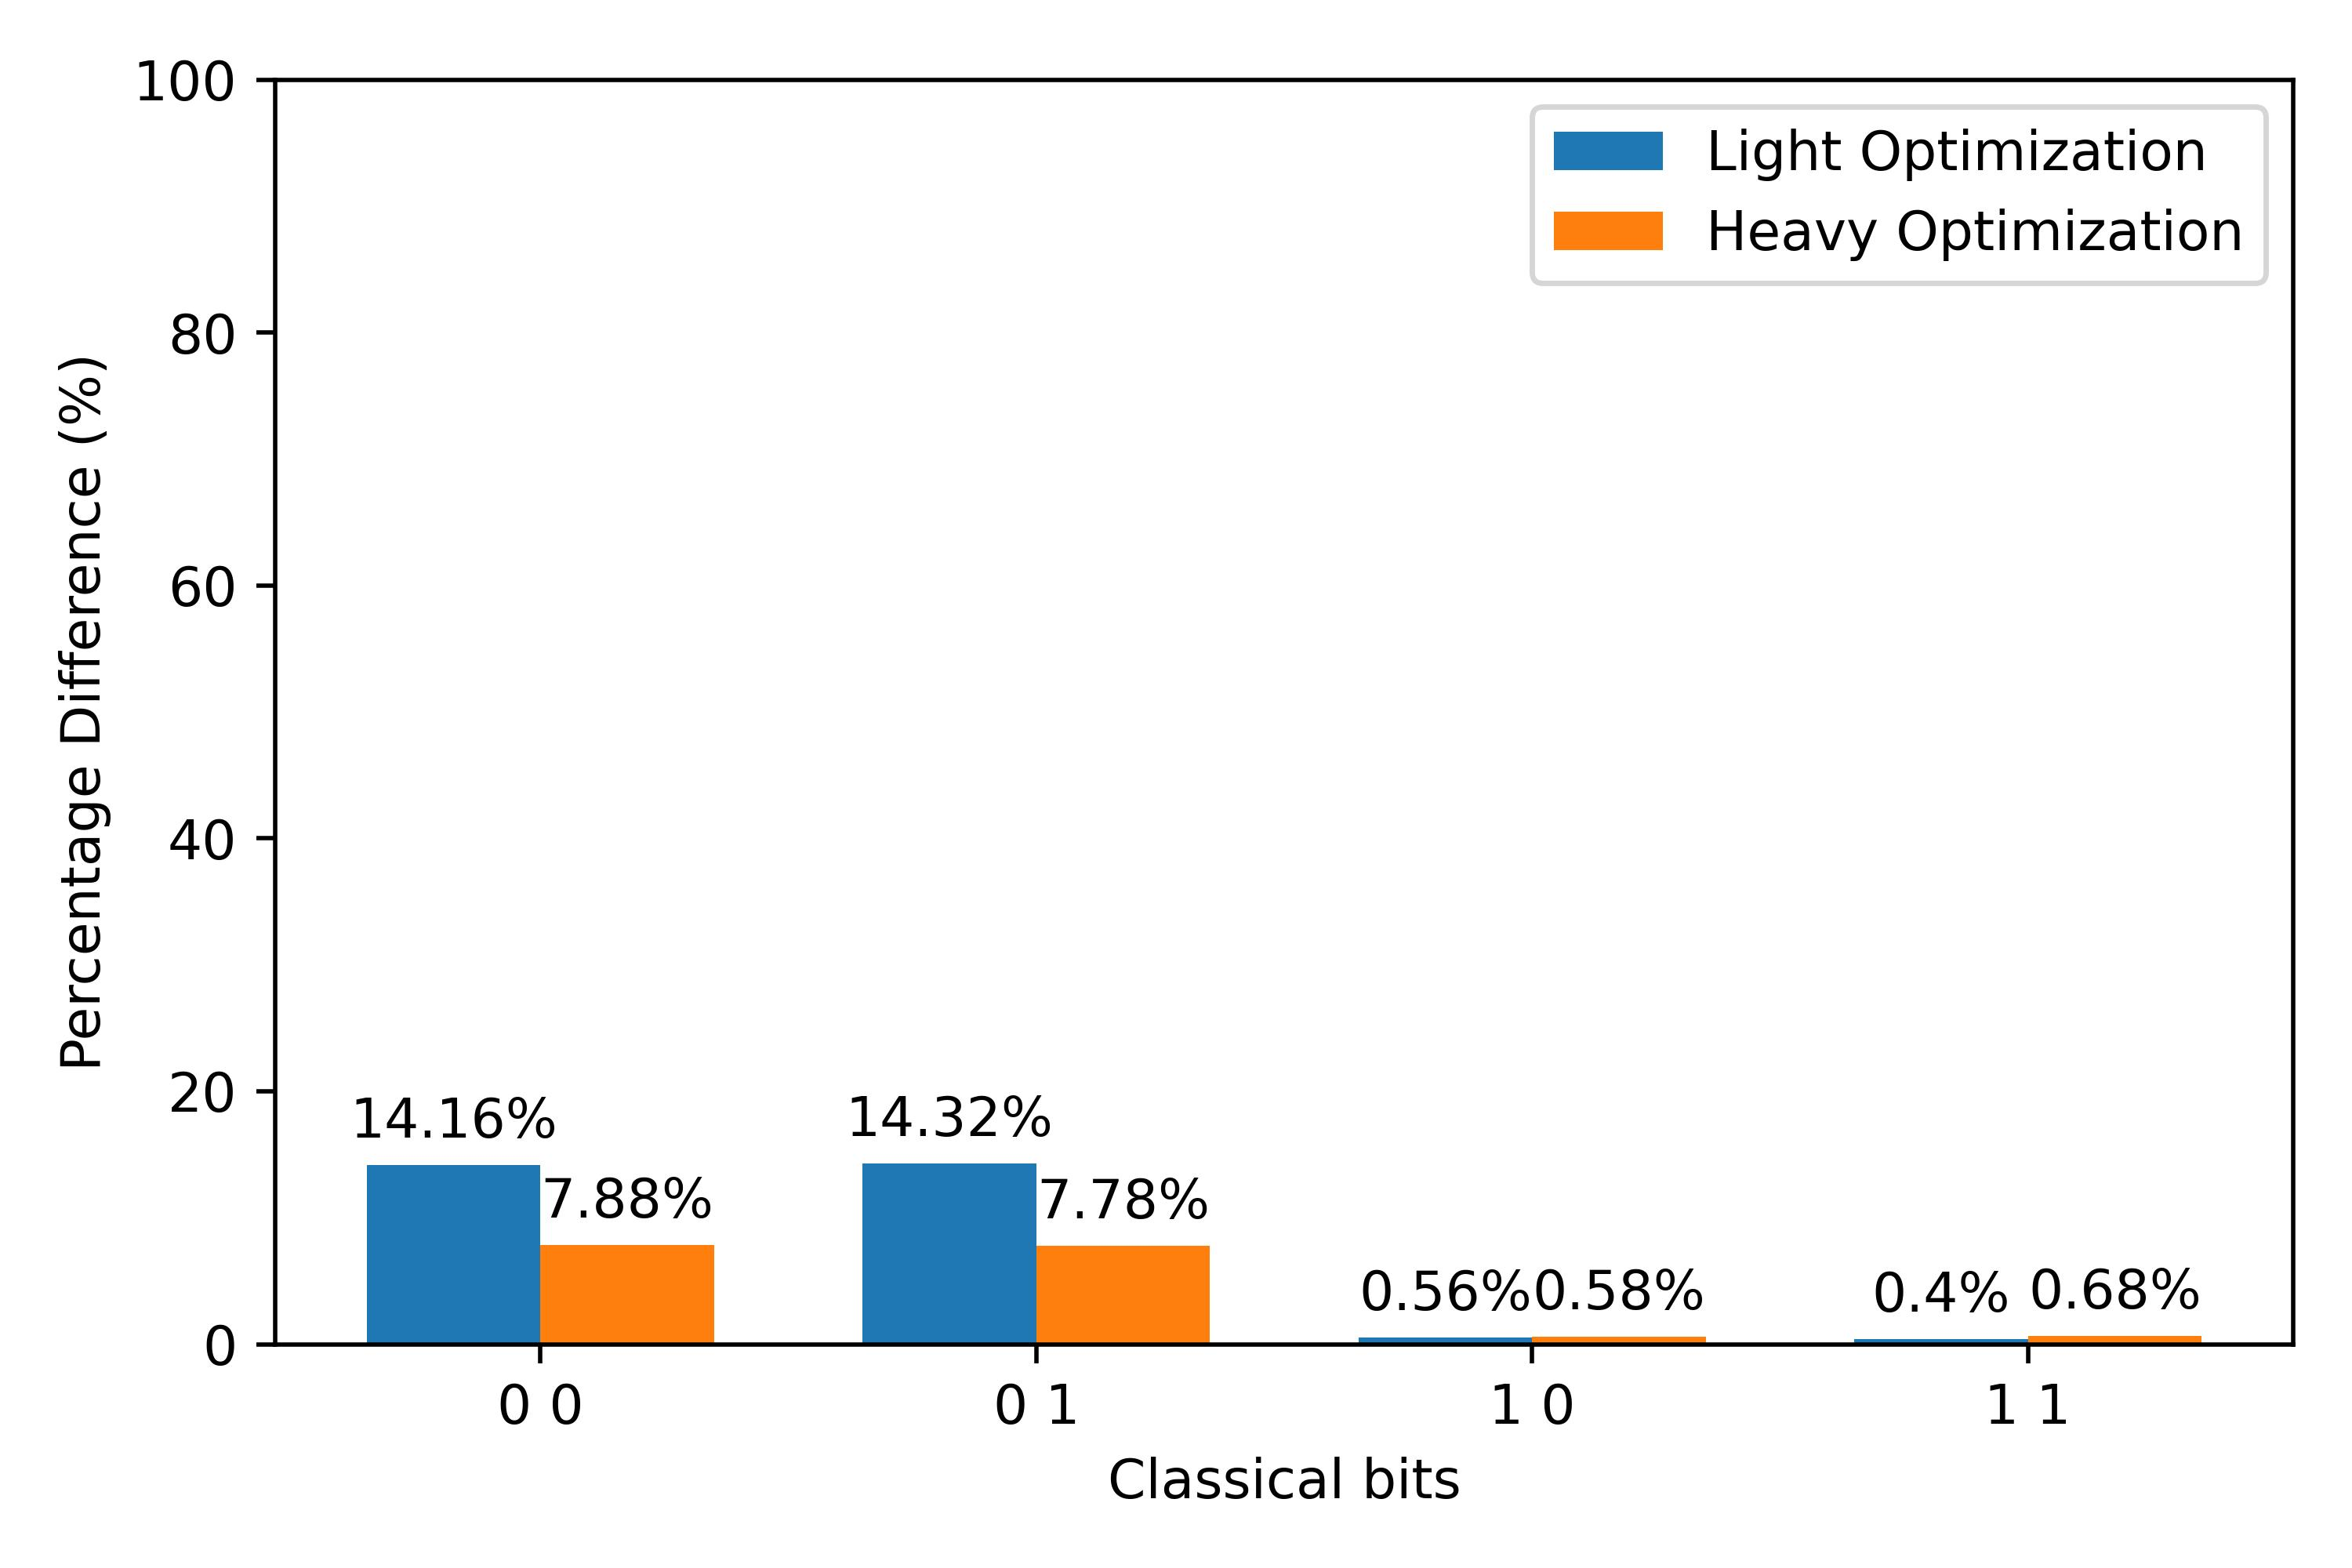
\includegraphics[width=\linewidth]{figures/po_repeated_post_swap.jpg}
    \caption{Repeated post swap}
    \label{fig:po_all_repeated_post_swap}
  \end{subfigure}
  \caption[Purification optimization results]{The results of experiments testing the differences of various purification protocols under different optimization schemes. The experiments were carried out for different purification strategies.}
  \label{fig:po_all}
\end{figure}
There were 20 independent measurement results obtained from 20 iterations of the circuit runs per purification strategy. The probabilities were then averaged for each purification strategy to get the estimate of the true probability. Those results were then used for each purification strategy, in finding the difference between Deutsch's and Bennett's estimate of probability under the light optimization scheme then the heavy optimization scheme before plotting them as is in Figure \ref{fig:po_all}. The differences were plotted as percentages.

The classical bits represent the classical states that can be measured by Alice and Bob at the end of the communication channel. The lower the percentage values, the lower the difference in the measurement results between Deutsch's and Bennett's purification protocol executed under the indicated optimization scheme. This is to mean that the near zero percentages show that the purification protocols under consideration would give similar measurement results.

The results from this experiment clearly show and confirm that the choice of purification protocol has on the average minimal impact on the overall purification optimization scheme used in the purification circuits. However minimal the impact, they should still be attended to and monitored given that some purification strategies do have higher percentage values such as Figure \ref{fig:po_all_post_swap} and \ref{fig:po_all_repeated_post_swap}.
%The most important bits are the 00 since they represent the expected ideal measurement results, with the rest of the bits representing states that are the result of noise in the circuit.
%Note also that in the bits 00, the percentage differences are quite minimal.
%%%%%%%%%%%%%%%%%%%%%%%%%%%%%%%%%%%%%%%%%%%%%%%%%%%%%%%%%%%%%%%
%%%%%%%%%%%%%%%%%%%%%%%%%%%%%%%%%%%%%%%%%%%%%%%%%%%%%%%%%%%%%%%
% \clearpage
\section{Conclusions}
In this study, we have presented a quantum repeater design setup and implementation that provides insight into determining the optimum strategy for conducting entanglement purification. The presented circuit architecture has been used to investigate purification strategies and the impact of optimization schemes applied under the two purification protocols for near-term quantum repeaters.

Four purification strategies were tested using Deutsch's purification protocol. Our results showed that the post Bell-pair and the pre-and-post swap strategies presented the most favourable strategies in the quantum repeater protocol.

Importantly, the various optimization levels had minimal impact on the performance of the purification protocols. The optimization schemes don't necessarily favour a certain purification protocol.

Our research has demonstrated that combining various approaches can yield a significant improvement in the performance of quantum repeaters, leading to better efficiency in the operation of future practical quantum repeaters.


%%%%%%%%%%%%%%%%%%%%%%%%%%%%%%%%%%%%%%%%%%
\subsection*{Code Availability}
All the code written for our research necessary to reproduce our results is available on GitHub \cite{karokigithub}.


\bibliographystyle{unsrt}
% \bibliography{references} % see references.bib for bibliography management



\begin{thebibliography}{00}
    \bibitem{Bennett_1993}
    {Charles H. Bennett, Gilles Brassard, Claude Cr\'epeau, Richard Jozsa, Asher Peres, and  William K. Wootters}.
    {Teleporting an unknown quantum state via dual classical and Einstein-Podolsky-Rosen channels}.
    {\sl Phys. Rev. Lett.},
    {70}:
    % {13},
    {1895--1899},
    % {0},
    {Mar}
    {1993}.
    {American Physical Society},
    % {DOI{10.1103/PhysRevLett.70.1895}},
    {\url{https://link.aps.org/doi/10.1103/PhysRevLett.70.1895}}

    \bibitem{Ruihong_2019}
    {Qiao Ruihong and Meng Ying}.
    {Research Progress Of Quantum Repeaters}.
    {\sl Journal of Physics: Conference Series},
    {1237},
    % {5},
    {jun}
    {2019},
    {{IOP} Publishing},
    % {10.1088/1742-6596/1237/5/052032},
    {\url{https://doi.org/10.1088/1742-6596/1237/5/052032}}

    \bibitem{Briegel_1998}
    {H.-J. Briegel, W. D\"ur, J. I. Cirac and P. Zoller, }.
    {Quantum Repeaters: The Role of Imperfect Local Operations in Quantum Communication}.
    {\sl Phys. Rev. Lett.},
    {81}:
    % issue = {26},
    {5932--5935},
    % numpages = {0},
    {Dec}
    {1998},
    {American Physical Society},
    % doi = {10.1103/PhysRevLett.81.5932},
    {\url{https://link.aps.org/doi/10.1103/PhysRevLett.81.5932}}

    \bibitem{Das_2021}
    {Sowmitra Das, Md. Saifur Rahman, and Mahbub Majumdar}.
    {Design of a Quantum Repeater Using Quantum Circuits and Benchmarking Its Performance on an IBM Quantum Computer}.
    {\sl Quantum Information Processing},
    {20}:
    % {7},
    {1570-0755},
    {Jul 2021},
    {Kluwer Academic Publishers},
    {USA},
    {\url{https://doi.org/10.1007/s11128-021-03189-8}}
    % {10.1007/s11128-021-03189-8},

    \bibitem{Gisin_2007}
    {Nicolas Gisin and Rob Thew}.
    {Quantum communication}.
    {\sl Nature Photonics},
    {1},
    % {3},
    {2007},
    % doi={10.1038/nphoton.2007.22},
    {\url{https://doi.org/10.1038/nphoton.2007.22}} 
    
    \bibitem{Herbst_2015}
    {Thomas Herbst, Thomas Scheidl, Matthias Fink, Johannes Handsteiner, Bernhard Wittmann, Rupert Ursin and Anton Zeilinger }.
    {Teleportation of entanglement over 143 km}.
    % {https://doi.org/10.48550/arXiv.1403.0009}
    {2015},
    {\sl arXiv},
    {\url{https://arxiv.org/abs/1403.0009}}
    
    \bibitem{Muralidharan2016}
    {Sreraman Muralidharan, Linshu Li, Jungsang Kim, Norbert Lütkenhaus, Mikhail D. Lukin and  Liang Jiang}.
    {Optimal architectures for long distance quantum communication}.
    {\sl Scientific Reports},
    {Feb}
    {2016},
    {6},
    {\url{https://doi.org/10.1038/srep20463}}    

    \bibitem{Bennett_1996}
    {Charles H. Bennett, Gilles Brassard, Sandu Popescu, Benjamin Schumacher, John A. Smolin, and William K. Wootters}.
    {Purification of Noisy Entanglement and Faithful Teleportation via Noisy Channels}.
    {\sl Phys. Rev. Lett.},
    {76}:
    % issue = {5},
    {722--725},
    % numpages = {0},
    {Jan}
    {1996},
    {American Physical Society},
    % doi = {10.1103/PhysRevLett.76.722},
    {\url{https://link.aps.org/doi/10.1103/PhysRevLett.76.722}}    

    \bibitem{Deutsch_1996}
    {David Deutsch, Artur Ekert, Richard Jozsa, Chiara Macchiavello, Sandu Popescu, and  Anna Sanpera}.
    {Quantum Privacy Amplification and the Security of Quantum Cryptography over Noisy Channels}.
    {\sl Phys. Rev. Lett.},
    {77}:
    % issue = {13},
    {2818--2821},
    % numpages = {0},
    {Sep}
    {1996},
    {American Physical Society},
    % doi = {10.1103/PhysRevLett.77.2818},
    {\url{https://link.aps.org/doi/10.1103/PhysRevLett.77.2818}}
    
    \bibitem{Krastanov2019optimized}
    {Stefan Krastanov, Victor V. Albert, and Liang Jiang}.
    {Optimized {E}ntanglement {P}urification}.
    {\sl {Quantum}},
    {{Verein zur F{\"{o}}rderung des Open Access Publizierens in den Quantenwissenschaften}},
    {3}: {123},
    {2521-327X},
    {feb}
    {2019},
    % doi = {10.22331/q-2019-02-18-123},
    {\url{https://doi.org/10.22331/q-2019-02-18-123}}

    \bibitem{karokigithub}
    {Karoki A. Mugambi}.
    {Quantum Repeater Design},
    {Github, \url{https://github.com/Phystro/Quantum-Repeater-Design}},
    {2023},
    {\url{https://github.com/Phystro/Quantum-Repeater-Design}}
    
%%%%%%%%%%%%%%%%%%%%%%%%%%%%%%%%%%%%%%%%%%%%%%%%%%%%%%%%%%%%%%%%%%%%%%%%%%%%%%%%%%%%%%%%%    
    
\end{thebibliography}



\end{document}
